% \subsection{Impact of RPP on Repetition + Performance}

% \subsection{RAP enable tuning to obtain the trade-off between performance and repetition
% }

% \subsection{Compare the performance using tuned RPP (based on RAP)
% }

% \subsection{Further Discussions}

\subsection{Experimental settings}
\textbf{Datasets.} 
% \begin{table}[]
% \centering
% \caption{Datasets used in our experiments. The Size refers to the number of questions or samples in the test set. }
% \label{tab:dataset}
% \begin{tabular}{l|l|r}
% \toprule
% Dataset                & Task                & \multicolumn{1}{l}{Size} \\ \midrule
% \webqsp  & Knowledge Base QA   & 1008                     \\
% \ms     & Open-ended QA       & 500                      \\
% \mac    & Machine Translation & 1133                    \\ \bottomrule
% \end{tabular}
% \end{table}
We conduct the experiments using three datasets including \webqsp \cite{yih2016value} and \ms
% \footnote{\url{https://microsoft.github.io/msmarco/}}
\cite{bajaj2016ms, huang2024performance} for question answering (QA), and \mac \cite{huang2025optimizing} for Chinese-English machine translation (MT). The datasets contain 1,008, 500, and 1,133 testing questions, respectively. To perform RAG on \webqsp, we crawled relevant articles from Wikipedia, and retrieve 8 most relevant document chunks when answering each question for RAG prompting. We also adopt Gemini-1.0-Pro to evaluate for the knowledge base question answering task (KBQA) where the ground-truth answers contains lists of entities instead of natural language text. More details of the dataset and LLM-based KBQA evaluation are presented in the Appendix (\ref{sec:data}). 

% as detailed in Section \ref{sub:data-col-pre}.

% \noindent
% \textbf{Open-source LLMs.} We evaluate nine open-source LLMs including Llama-2 (7B, 13B, 70B), Llama-3 (8B, 70B), Gemma-1.1 (2B, 7B), Phi-3-mini (3.8B), and Mistral-7B. These are currently some of the most popular open-source LLMs suitable for use in commercial applications (permitted by their licenses).
% \textbf{Open-source LLMs.} \new{
% \new{Table \ref{tab:ai_models} provides an overview of all the models utilized in our study, detailing their companies, model names, and corresponding HuggingFace model identifiers. 
% For QA tasks, we evaluate nine open-source LLMs, including Llama-2 (7B, 13B, 70B), Llama-3 (8B, 70B), Gemma-1.1 (2B, 7B), Phi-3-mini (3.8B), and Mistral-7B. For MT task, we evaluate three open-source LLMs: Phi-3.5-mini (3.8B), Mistral-7B, and Llama-3.1-70B. These models are among the most popular open-source LLMs suitable for use in commercial applications, as permitted by their respective licenses. More details can be found in the Appendix (\ref{subsec:overview_llms}). %\ref{subsec:overview_llms}.
% }
\textbf{Open-Source LLMs.} This study evaluates a diverse set of open-source large language models (LLMs) for question answering (QA) and machine translation (MT) tasks. For QA, we assess nine models: Llama-2 (7B, 13B, 70B), Llama-3 (8B, 70B), Gemma-1.1 (2B, 7B), Phi-3-mini (3.8B), and Mistral-7B. For MT, we evaluate three models: Phi-3.5-mini (3.8B), Mistral-7B, and Llama-3.1-70B.

Table~\ref{tab:ai_models} provides an overview of these models, including their respective companies, model names, Hugging Face identifiers, and the tasks they were evaluated on. This selection spans a broad range of model sizes and architectures, representing the state of the art in open-source LLM development. These models are widely used in commercial applications under their respective licenses.

The diversity of this selection enables a robust comparison across model families and sizes, offering insights into the relative strengths of different open-source LLMs in QA and MT tasks.

\begin{table*}[htbp]
\caption{Overview of Large Language Models and Their Specifications by Task}
\label{tab:ai_models}
\centering
\resizebox{.8\textwidth}{!}{
\begin{tabular}{l|l|l|l}
\toprule
\textbf{Company} & \textbf{Model Name} & \textbf{Hugging Face Model ID} & \textbf{Task} \\
\midrule
\multirow{6}{*}{Meta} 
& Llama-2-7B & meta-llama/Llama-2-7b-chat & QA \\
& Llama-2-13B & meta-llama/Llama-2-13b-chat & QA \\
& Llama-2-70B & meta-llama/Llama-2-70b-chat & QA \\
& Llama-3-8B & meta-llama/Meta-Llama-3-8B-Instruct & QA \\
& Llama-3-70B & meta-llama/Meta-Llama-3-70B-Instruct & QA \\
& Llama-3.1-70B & shenzhi-wang/Llama3.1-70B-Chinese-Chat & MT \\
\midrule
\multirow{2}{*}{Microsoft} 
& Phi-3-mini & microsoft/Phi-3-mini-128k-instruct & QA \\
& Phi-3.5-mini & microsoft/Phi-3.5-mini-instruct & MT \\
\midrule
\multirow{2}{*}{Google} 
& Gemma-1.1-2B & google/gemma-1.1-2b-it & QA \\
& Gemma-1.1-7B & google/gemma-1.1-7b-it & QA \\
\midrule
\multirow{2}{*}{Mistral AI} 
& Mistral-7B-v0.2 & mistralai/Mistral-7B-Instruct-v0.2 & QA \\
& Mistral-7B-v0.3 & shenzhi-wang/Mistral-7B-v0.3-Chinese-Chat & MT \\
\bottomrule
\end{tabular}
}
\end{table*}

\textbf{Automating QA and MT Tasks with LLMs.} 
We developed a Python script specifically designed to evaluate the performance of LLMs on QA and MT tasks. The script leveraged the open-source HuggingFace Transformers library~\cite{wolf2020transformers} and was executed across all models and datasets. For QA tasks, an RPP range of 1.0 to 1.3 was applied, while for MT tasks, an RPP range of 1.0 to 1.1 was used, both with increments of 0.02. To ensure consistency and reproducibility across experiments, the temperature was set to 0 and \texttt{top\_p} was fixed at 0.95.
% \noindent
% \textbf{Automated Question Answering with LLMs:} 
% \textbf{\new{Automated Answer Generation with LLMs:}} 
% \new{We developed Python scripts to automate interactions with LLMs for generating answers. The scripts were applied to all models and datasets, with the \rp ranging from 1.0 to 1.1 for MT task and up to 1.3 for QA tasks, incremented by 0.02.}
% We developed a Python script leveraging LangChain and HuggingFace Transformers\footnote{\url{https://huggingface.co/docs/transformers/en/index}} to automate interactions with LLMs for generating answers to questions in the datasets. The script was executed using all models and both datasets, with a repetition penalty ranging from 1.0 to 1.3 in increments of 0.02. 
% We developed a Python script to automate interactions with LLMs for generating answers. The script was run on all models and datasets, applying \rp ranging from 1.0 to 1.3 in 0.02 increments.

% The questions and generated answers, along with other data elements from the datasets, were stored in CSV files for further data processing, such as detecting repetitions and evaluating performance.

% \noindent
\textbf{Prompt Templates:} 
To investigate LLMs’ behaviors under different prompting strategies, we implemented three QA prompt templates: (1) \textit{RAG - Generic Prompt} (\raggen): a uniform basic template for all models; (2) \textit{RAG - Chat Template} (\ragtem): LangChain’s default template tailored to each LLM’s chat format, maintaining the same core content; and (3) \textit{Non-RAG}: simulates a single-turn conversation in the LLM’s chat format.
For MT, we used two templates: (1) \textit{MT - Generic Prompt} (\mtgen): a basic template applied uniformly, and (2) \textit{MT - Chat Template} (\mttem): a template designed for each LLM’s chat format. Prompt templates are shown in the Appendix (\ref{sec:prompt}). 

% To investigate LLMs’ behaviors under different prompting strategies, we implemented three prompt templates \new{for QA}: (1) \textit{RAG - Generic Prompt} (\raggen): using the same basic prompt template for all the models.
% (2) \textit{RAG - Chat Template} (\ragtem): using LangChain’s default template to match each LLM’s chat format. While the template varies across model families, the main message content remains the same. 
% (3) \textit{Non-RAG}: simulates a single-turn conversation between a human and the LLM, following the LLM’s chat format. 
% \new{For MT, we implemented two prompt templates: 
% (1) \textit{MT - Generic Prompt} (\mtgen): a basic prompt template applied uniformly across all models, and 
% (2) \textit{MT - Chat Template} (\mttem): using the template to fit each LLM’s chat format.} 
%
% The prompt templates for Llama-3 models is shown in the Appendix. 

% The Non-RAG prompt for Llama-3 models is shown in Listing \ref{list:non-rag} in Appendix.

% \noindent
\textbf{Evaluation Metrics:} For \webqsp, we use \textit{precision}, \textit{recall}, and \textit{F1} scores. For \mds, \new{we employ BERTScore~\cite{zhang2019bertscore}, using deberta-xlarge-mnli model to ensure optimal performance, as it provides the highest correlation with human evaluations. Results are reported as the average F1 score across the entire dataset, referred to as \textit{BERT-F1}. 
For \mac, we employ the Crosslingual Optimized Metric for Evaluation of Translation (\textit{COMET}), a neural-based evaluation metric that leverages contextual embeddings from pretrained language models to assess translation quality~\cite{rei2022comet}. COMET has demonstrated strong correlation with human judgments, making it a reliable metric for translation evaluation.}
%we use ROUGE-L~\cite{lin2004rouge,joshi2023deepsumm} and BLEU-1~\cite{dey2022evaluating} to assess answer quality. 
%
For repetition evaluation, we report the repetition ratio (Equation \ref{eq:rr_dataset}).
%We also introduce an overall performance score, denoted as \hm and calculated as the harmonic mean of BLEU-1 and ROUGE-L.
% : 
% \begin{align}
%     H = \frac{2 \times \text{BLEU-1} \times \text{ROUGE-L}}{\text{BLEU-1} + \text{ROUGE-L}} 
% \end{align}
We also report the \rap scores, applied on the corresponding evaluation metrics (Section \ref{sec:rap}).

% Existing metrics: What metrics for WebQSP, What metrics for MS Macro. 
% NEW: Repetition Factor
% NEW: Repetition Factor Adjusted Perf Scores



% \begin{itemize}
%     \item Investigate the impact of \rp on repetition and performance 
%     \item \rf to incorporate repetition penalty in the performance so that we can perform hyperparamter tuning 
    
% \end{itemize}


% \noindent
% \textbf{Repetition Detection - Baseline Method} 
% To benchmark our proposed repetition detection method, we develop a baseline method based on \cite{Fu2020ATA} that identifies adjacent identical word phrases using a suffix array \cite{10.5555/320176.320218} sorted lexicographically. The method scans the suffix array in multiple passes, comparing row-adjacent phrases to find exact matches where their index distance equals the phrase length. A greedy approach is then used to extract the longest combination of adjacent repeated phrases. See Appendix for more details.
% To benchmark our proposed repetition detection method, we develop a baseline method based on \cite{Fu2020ATA} to identify adjacent identical word phrases. To simulate this, tokenized words of the input text are stored in a suffix array \cite{10.5555/320176.320218}, which is sorted lexicographically. 
% For example, "This is repeated is repeated text" has 6 suffixes (Figure \ref{fig:suffix_array_simulation}) stored as indexes 1, 3, 2, 4, 5, 0. 
% To find repeated phrases, the method scans the suffix array in $N$ passes, where $N$ equals the size of tokenized words, comparing row-adjacent phrases of length 1 ... $N$. Phrases are considered repeating if they match exactly and their suffix array index distance equals the phrase length. A greedy approach is then used to extract the longest combination of adjacent repeated phrases. 
% An experimental result demonstrate that \alg is faster by 12\% compared to the baseline method and performs comparably better than the baseline algorithm. Moreover, the method discovers abnormalities in the text that were not addressed by the baseline method, details of which will be provided in section \ref{subsec:evaluating-text-abnormalities}. 



% \textbf{Findings}
% \begin{enumerate}
%     \item Chat template significantly reduce repetition. It's not well-known/common practice by developers to use Chat template, in LLM application development. 
%     \item For generic prompt, increasing RPP normally reduce repetition. With Chat template model, the impact of \rpp is not as effective, for some model, increasing too high RPP can lead to higher repetition 
%     \item We show that RPP also have impact on the performance, so a balance approach can be achieved with RAP (with minimal findings)
% \end{enumerate}

% \textbf{Experiments}
% \begin{enumerate}
%     \item Impact of RPP on Repetition and Performance: showing results of all models, all datasets, all prompts. (@Donghao)
%     \item Optimizing the trade-off between performance and repetition. Objective is to show how to tune \rpp using RAP. (Existing content, maybe shorten). Remove numbers, change MTR to RR. Add for MT (@Donghao) 
%     \item comparing the best original + \rap of all models. The figures combining of figure-1-like figures. 
%     \item What is the percentages of responses having repetition, if having repetition, how severe it is? Choose few models and show the results. 
% \end{enumerate}



% \begin{align}
%     Gain = \frac{RR_{Origin} - RR_{RAP}}{P_{origin} - P_{RAP}}
% \end{align}

\subsection{Impact of \rpp on Repetition and Performance}
\label{subsec:impact_of_rpp}
\begin{figure*}[ht!]
    \centering
    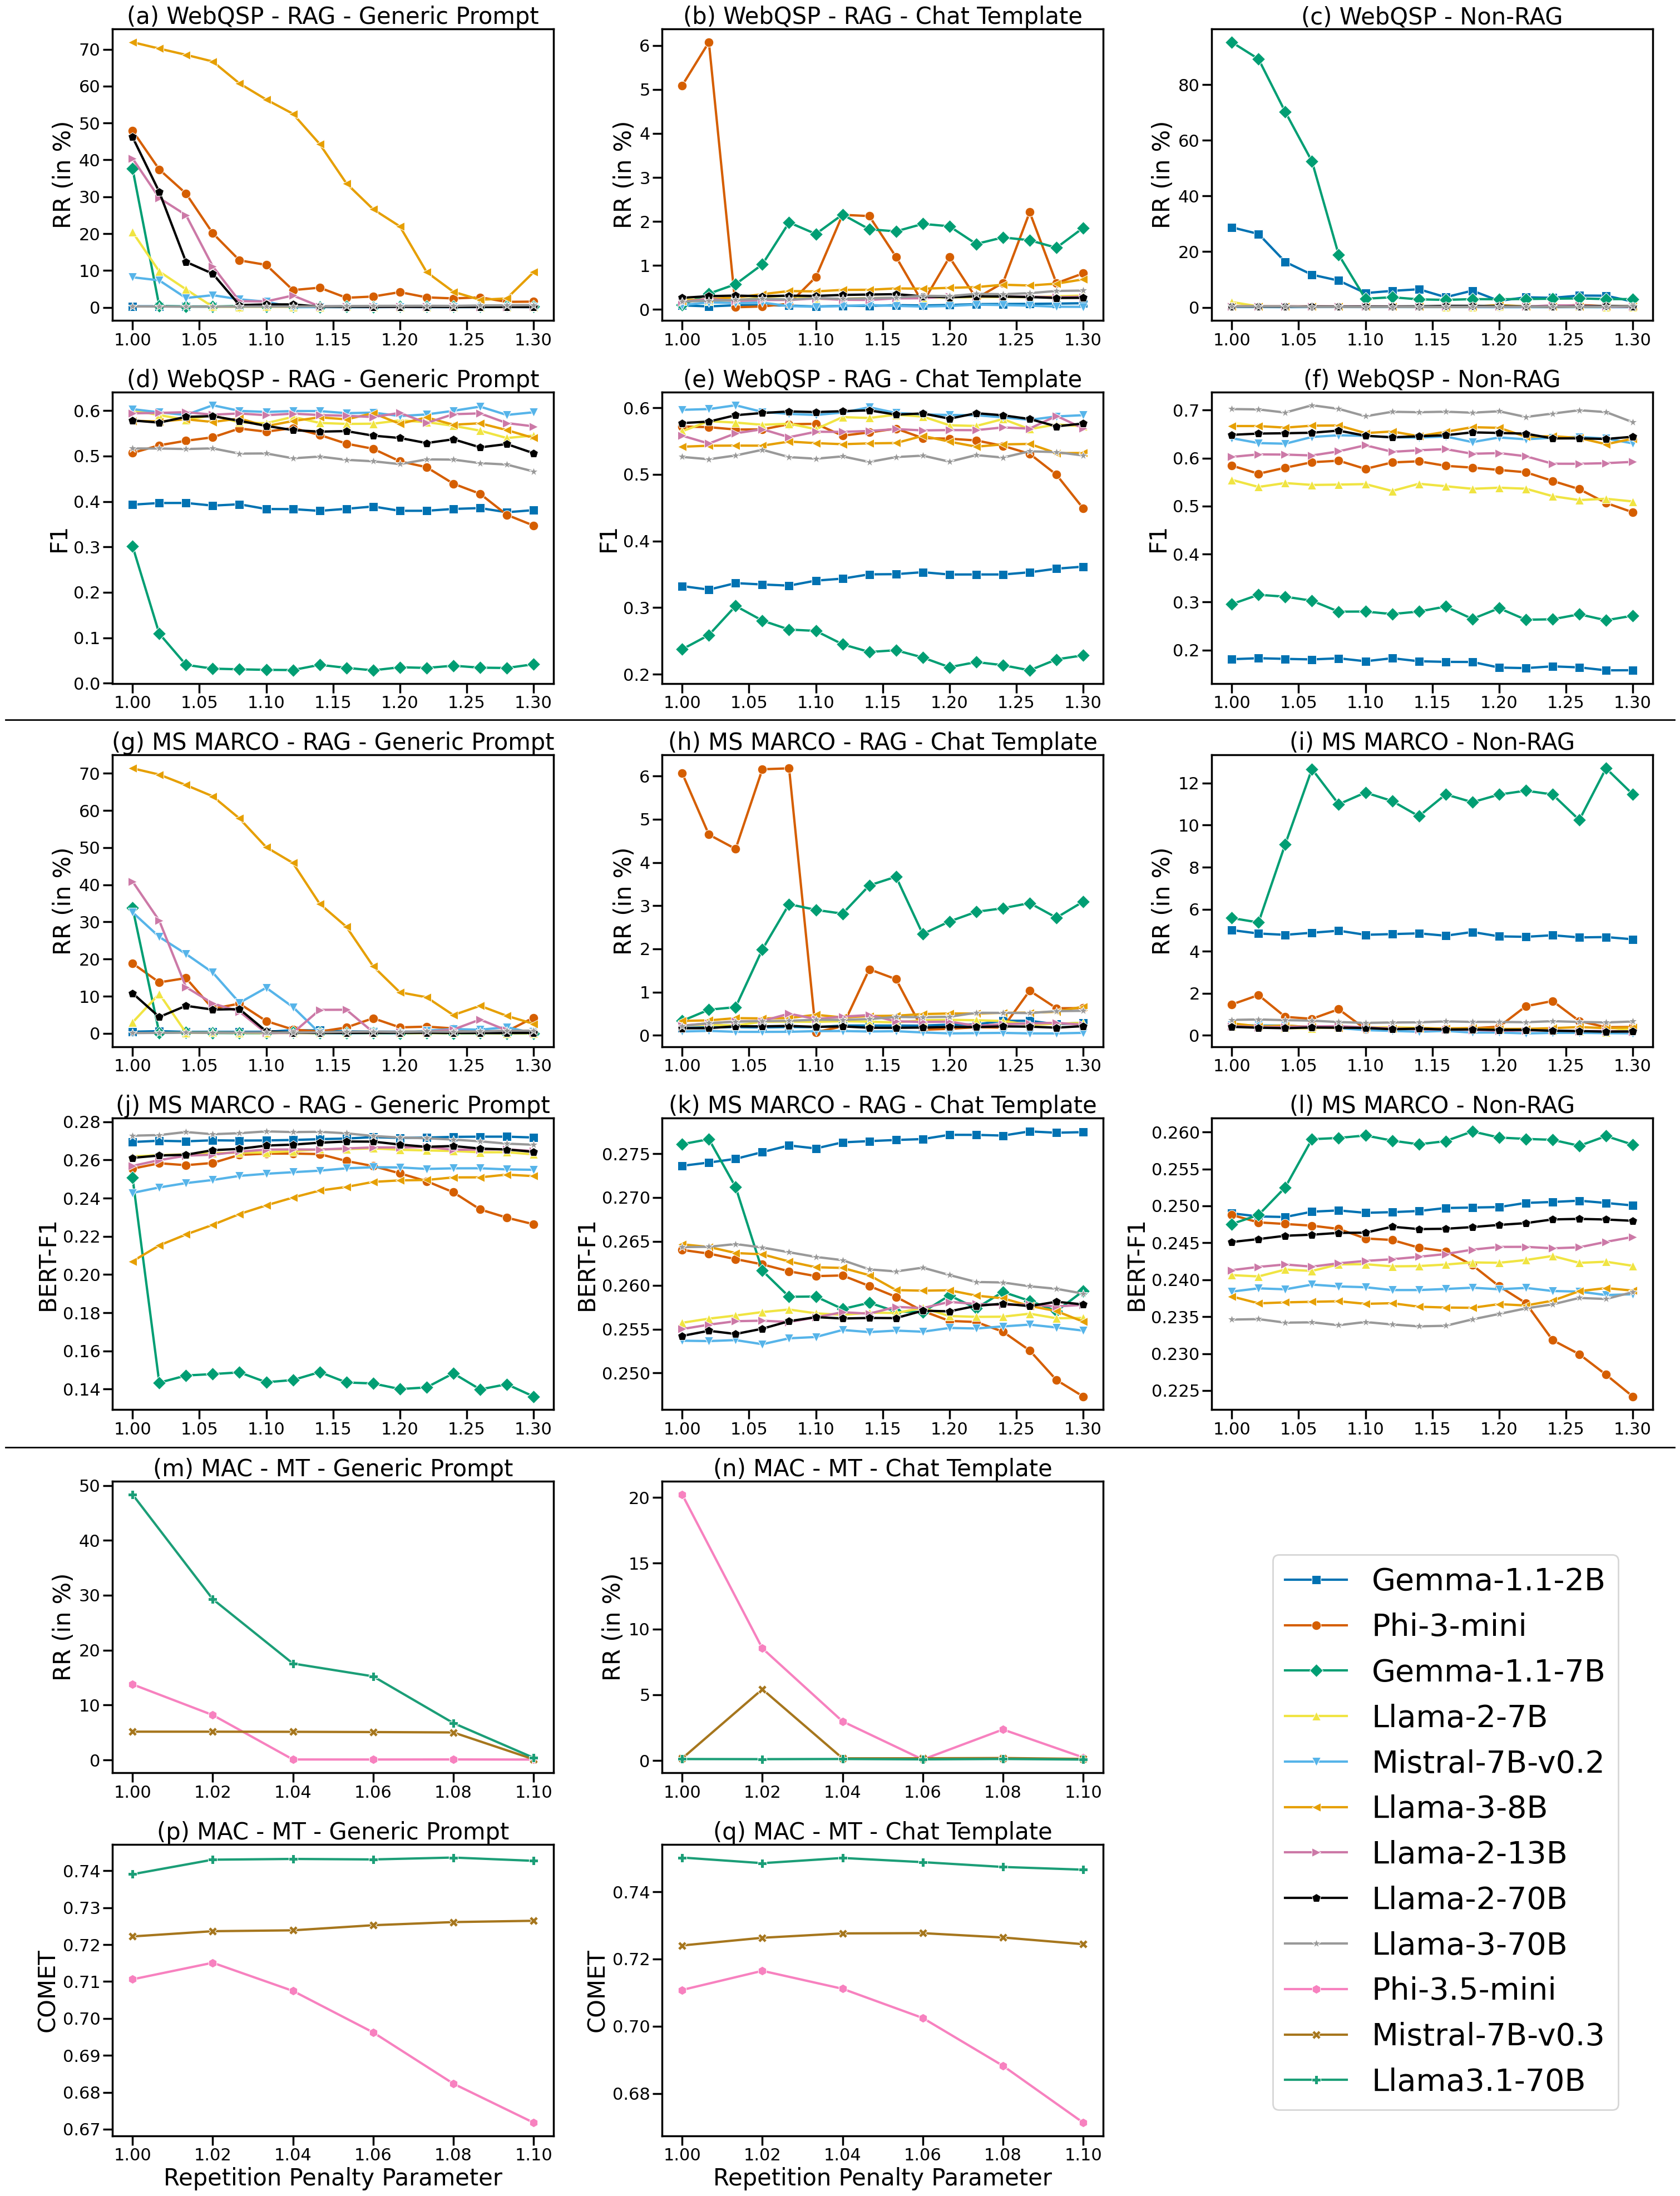
\includegraphics[width=\textwidth]{image/all-metrics-across-models_v2.png}
    \caption[Performance and Repetition Metrics Across Models]{
    Illustrating the impact of \rpp on \rr and performance across models, datasets, and prompting strategies. 
    % Results highlight the effectiveness of Chat Templates in reducing repetition while maintaining competitive performance, as well as the diminishing returns of increasing RPP beyond certain thresholds.
    % Performance and \rr when varying \rpp. This figure illustrates the impact of \rpp on repetition (RR) and performance (F1, BERT-F1, COMET) across different models, datasets (WebQSP, MS MARCO, MAC), and prompting strategies. Results highlight the effectiveness of Chat Templates in reducing repetition while maintaining competitive performance, as well as the diminishing returns of increasing RPP beyond certain thresholds.
    %\todo{to make subfigure title much bigger, can we draw a line between datasets?}
    }
    \label{fig:all-metrics-across-models_v2}
\end{figure*}

Figures \ref{fig:all-metrics-across-models_v2} illustrates the impact of \rpp on the repetition and performance of different open-source LLMs on the three datasets, using different prompting strategies. 
The results show that increasing RPP generally reduces repetition across strategies and datasets but often leads to a decline in performance. The trending and severity vary by model; for instance, while Phi-3-mini’s performance on MS MARCO-RAG-GP dropped significantly with RPP above 1.14, Llama-3-8B showed improved performance with higher RPP values under the same conditions. 
% The trade-off between reducing repetition and maintaining accuracy becomes evident beyond 1.15–1.20.
Therefore, selecting an optimal RPP value is crucial to balance repetition reduction with minimal impact on performance.
% metrics like F1, BERT-F1, or COMET.
%dataset

The datasets also show different behaviors. WebQSP generally exhibits higher repetition levels (e.g., at RPP = 1.0) than MS MARCO, especially with the RAG-GP strategy. This indicates that the nature of the dataset and task also influence repetition tendencies. In MAC dataset, despite a smaller RPP range tested, repetition still decreases as RPP increases. For both QA datasets, the Chat Template strategy consistently reduces repetition, showing lower RR values than the Generic Prompt approach. This suggests that the Chat Template effectively minimizes repetition in QA tasks. However, it surprisingly does not offer the same benefit for MT task, where increasing RPP effectively reduces repetition.



% Unlike QA tasks, the Chat Template and Generic Prompt strategies show similar repetition levels in MT.

% Chat template 
% Impact of RPP 
% , but Llama-3-8B in the same setting gets higher performance with higher value of RPP. 

% Several key insights can be drawn from these results:

% \noindent 
% \textbf{Chat Template Superiority}: 
% Across both QA datasets and all RPP values, the Chat Template strategy consistently achieves the lowest levels of repetition. This is reflected in lower RR values compared to the Generic Prompt approach. These results suggest that using a Chat Template is an effective method for minimizing repetitive content in model outputs for QA task. Supperisingly, using template does not seem to help for machine translation, although repetition can be reduced easily by increasing \rpp for this task. 

% \noindent 
% \textbf{The impact of RPP}: the results show that increasing RPP generally reduces repetition across different strategies and datasets. 
% However, it is also shown that using higher RPP value often leads to a decline in performance for most of the models and settings. The severity of the impact varies depending on the model. For example, Phi-3-mini's performance in MS MARCO-RAG-Generic Prompt significantly reduced when using RPP higher than 1.14.
% The impact is particularly noticeable as RPP increases beyond 1.15--1.20, where the trade-off between reducing repetition and maintaining model accuracy becomes evident. Therefore, it is important to choose an optimal RPP value that balances the reduction in repetition with minimal impact on performance (F1, BERT-F1, or COMET).
% \noindent \textbf{Diminishing Returns}: For most strategies, the reduction in repetition plateaus as RPP increases beyond certain thresholds (typically around 1.20--1.25). This indicates that there may be an optimal range for RPP settings, beyond which further increases provide minimal additional benefits in terms of repetition reduction. 

% \noindent \textbf{Dataset Differences}: The behaviors are also different in the different datasets. WebQSP dataset generally exhibits higher baseline repetition levels (at RPP = 1.0) compared to MS MARCO, particularly for the RAG - Generic Prompt strategy. This indicates that the nature of the dataset and task can significantly influence repetition tendencies. In the MAC machine translation (MT) task, although a smaller range of RPP values was tested, repetition reduction is still evident as RPP increases. Interestingly, unlike the QA tasks, the Chat Template and Generic Prompt strategies show comparable levels of repetition in the MT task.

% These findings highlight the importance of carefully tuning the RPP and selecting appropriate prompting strategies to optimize model performance while minimizing undesirable repetition. The results also underscore the effectiveness of Chat Templates in managing repetition across different models and datasets.

% Figure \ref{fig:mean-metrics-across-models} shows the results of average mean total repetitions and performance when varying \rp.  


% \textbf{Mean Total Repetitions:} Increasing RPP generally reduces mean total repetitions across all models and prompt templates, indicating that a higher RPP effectively suppresses repetitive content. The \raggen exhibits the highest repetition issues, with mean total repetitions exceeding 600 at an RPP of 1.0, gradually decreasing as RPP increases. Repetition issues generally cease when RPP is greater than or equal to 1.2, a trend consistent across other prompt templates.

% \textbf{Performance Metrics}: For the WebQSP dataset (Figures \ref{fig:mean-metrics-across-models}a and \ref{fig:mean-metrics-across-models}c), increasing RPP stabilizes or slightly reduces F1 scores for \raggen and \ragtem, while Non-RAG methods maintain relatively stable F1 scores. For the MS MARCO dataset (Figures \ref{fig:mean-metrics-across-models}b and \ref{fig:mean-metrics-across-models}d), overall performance declines with increasing RPP for \raggen and \ragtem, while Non-RAG methods remain stable.




% \textbf{Mean Total Repetitions:} Increasing RPP generally reduces mean total repetitions across all models and prompt templates, indicating that a higher RPP effectively suppresses repetitive content. The \raggen exhibits the highest repetition issues, with mean total repetitions exceeding 600 at an RPP of 1.0, gradually decreasing as RPP increases. Repetition issues generally cease when RPP is greater than or equal to 1.2, a trend consistent across other prompt templates.

% \textbf{Performance Metrics:} For the WebQSP dataset (Figures \ref{fig:mean-metrics-across-models}a and \ref{fig:mean-metrics-across-models}c), increasing RPP tends to stabilize or slightly reduce F1 scores for \raggen and \ragtem. Non-RAG methods maintain relatively stable F1 scores across different RPP values. Conversely, for the MS MARCO dataset (Figures \ref{fig:mean-metrics-across-models}b and \ref{fig:mean-metrics-across-models}d), overall performance gradually declines with increasing RPP for \raggen and \ragtem, while Non-RAG methods exhibit greater stability.




% Interestingly, for WebQSP, Non-RAG methods provide the highest F1 scores across all RPP values, whereas for MS MARCO, they yield the lowest overall performance scores. This discrepancy likely arises from using BLEU-1 and ROUGE-L metrics for MS MARCO, which have lower correlation with human ratings \cite{clinciu2021study}, penalizing human-like LLM responses. Future work will explore embedding-based evaluation methods, like BERTScore and BLEURT, which correlate better with human ratings.
% While general trends in Figure \ref{fig:mean-metrics-across-models} are consistent across most models, several notable exceptions are identified. 
% Phi-3-mini Model with \ragtem (WebQSP and MS MARCO): Beyond an RPP of 1.24, total repetitions increase significantly (Figures \ref{fig:webqsp-metrics}b and \ref{fig:ms-marco-metrics}b), deviating from the expected trend. This model shows a sudden increase in answer length and text abnormalities beyond an RPP of 1.24.
% Phi-3-mini Model with Non-RAG Template (MS MARCO): Increasing RPP beyond 1.2 results in a sharp rise in total repetitions (Figure \ref{fig:ms-marco-metrics}c), indicating sensitivity to higher RPP values. This model also shows increased answer length and text abnormalities.
% Gemma-1.1-7b Model with Non-RAG Template (MS MARCO): Total repetitions increase significantly beyond an RPP of 1.04 and do not decrease with further RPP increases (Figure \ref{fig:ms-marco-metrics}c), suggesting ineffective repetition suppression. This model shows increased newline and space repetitions beyond an RPP of 1.04, as it tries to format answers in bullet points. Additional details are in Appendix \ref{app:impact_of_rpp}.
% The impact of RPP on repetition and performance varies across models and prompting strategies. While increasing RPP generally reduces repetitions, it can also negatively affect performance metrics like F1 scores. RAG methods, especially using the Generic Prompt, exhibit significant fluctuations, necessitating careful tuning to balance repetition suppression with maintaining high performance quality.






% % Please add the following required packages to your document preamble:
% \usepackage{multirow}
\begin{table*}[t]
\centering
\resizebox{.85\textwidth}{!}{
\begin{tabular}{l|l|rrrr|rrrr|rrrr}
\toprule
\multirow{2}{*}{Dataset}   & \multirow{2}{*}{Model} & \multicolumn{4}{c|}{RAG - Generic Prompt}                                                                & \multicolumn{4}{c|}{RAG - Chat Template}                                                                 & \multicolumn{4}{c}{Non-RAG}                                                                             \\ \cline{3-14} 
                           &                        & \multicolumn{1}{c}{RPP} & \multicolumn{1}{c}{MTR} & \multicolumn{1}{c}{Perf.} & \multicolumn{1}{c|}{RAP} & \multicolumn{1}{c}{RPP} & \multicolumn{1}{c}{MTR} & \multicolumn{1}{c}{Perf.} & \multicolumn{1}{c|}{RAP} & \multicolumn{1}{c}{RPP} & \multicolumn{1}{c}{MTR} & \multicolumn{1}{c}{Perf.} & \multicolumn{1}{c}{RAP} \\ \hline
\multirow{18}{*}{WebQSP}   & Gemma-1.1-2B       & 1.04                    & 0.00                    & 39.7                    & 39.7                   & 1.30                    & 0.01                    & 36.1                    & 36.1                   & 1.20                    & 0.08                    & 16.3                    & 16.3                  \\\cmidrule{2-14}
                           % & Gemma-1.1-2B-F1           & 1.04                    & 0.00                    & 39.7                    & 39.7                   & 1.30                    & 0.01                    & 36.1                    & 36.1                   & 1.02                    & 51.67                   & 18.3                    & 10.2                  \\ \cmidrule{2-14}
                           & Gemma-1.1-7B       & 1.00                    & 35.46                   & 30.2                    & 18.2                   & 1.04                    & 0.09                    & 30.2                    & 30.1                   & 1.16                    & \textcolor{blue}{1.21}                    & 29.1                    & 27.7                  \\
                           & Gemma-1.1-7B-F1           & 1.00                    & 35.46                   & 30.2                    & 18.2                   & 1.04                    & 0.09                    & 30.2                    & 30.1                   & 1.02                    & \textcolor{blue}{633.61}                  & 31.5                    & 11.2                  \\\cmidrule{2-14}
                           & Llama-2-7B         & 1.06                    & \textcolor{blue}{0.01}                    & 58.9                    & 58.9                   & 1.16                    & 0.02                    & 59.0                    & 58.9                   & 1.00                    & 0.02                    & 54.8                    & 54.8                  \\
                           & Llama-2-7B-F1             & 1.00                    & \textcolor{blue}{78.48}                   & 60.1                    & 30.9                   & 1.16                    & 0.02                    & 59.0                    & 58.9                   & 1.00                    & 9.09                    & 55.5                    & 43.3                  \\\cmidrule{2-14}
                           & Llama-2-13B        & 1.20                    & 0.00                    & 59.5                    & 59.5                   & 1.28                    & 0.00                    & 58.8                    & 58.8                   & 1.10                    & 0.29                    & 62.7                    & 61.9                  \\
                           % & Llama-2-13B-F1            & 1.04                    & 62.02                   & 59.6                    & 32.1                   & 1.28                    & 0.00                    & 58.8                    & 58.8                   & 1.10                    & 0.29                    & 62.7                    & 61.9                  \\\cmidrule{2-14}
                           & Llama-2-70B        & 1.16                    & 0.00                    & 55.5                    & 55.5                   & 1.14                    & 0.03                    & 59.6                    & 59.5                   & 1.08                    & 0.19                    & 65.7                    & 65.2                  \\ \cmidrule{2-14}
                           % & Llama-2-70B-F1            & 1.06                    & 21.57                   & 58.8                    & 39.2                   & 1.14                    & 0.03                    & 59.6                    & 59.5                   & 1.08                    & 0.19                    & 65.7                    & 65.2                  \\\cmidrule{2-14}
                           & Llama-3-8B         & 1.26                    & \textcolor{blue}{9.96}                    & 57.2                    & 44.0                   & 1.18                    & 0.01                    & 55.8                    & 55.8                   & 1.06                    & 0.02                    & 66.8                    & 66.7                  \\
                           & Llama-3-8B-F1             & 1.18                    & \textcolor{blue}{178.99}                  & 59.4                    & 26.1                   & 1.18                    & 0.01                    & 55.8                    & 55.8                   & 1.08                    & 0.07                    & 66.8                    & 66.6                  \\\cmidrule{2-14}
                           & Llama-3-70B        & 1.06                    & 0.00                    & 51.7                    & 51.7                   & 1.06                    & 0.00                    & 53.7                    & 53.7                   & 1.06                    & 0.02                    & 71.0                    & 70.9                  \\
                           % & Llama-3-70B-F1            & 1.06                    & 0.00                    & 51.7                    & 51.7                   & 1.06                    & 0.00                    & 53.7                    & 53.7                   & 1.06                    & 0.02                    & 71.0                    & 70.9                  \\\cmidrule{2-14}
                           & Mistral-7B         & 1.26                    & 0.01                    & 60.9                    & 60.8                   & 1.04                    & 0.00                    & 60.4                    & 60.4                   & 1.08                    & 0.00                    & 64.8                    & 64.8                  \\
                           % & Mistral-7B-F1             & 1.06                    & 14.74                   & 61.2                    & 43.9                   & 1.04                    & 0.00                    & 60.4                    & 60.4                   & 1.08                    & 0.00                    & 64.8                    & 64.8                  \\\cmidrule{2-14}
                           & Phi-3-mini         & 1.16                    & 15.42                   & 52.7                    & 37.5                   & 1.08                    & 0.02                    & 57.5                    & 57.5                   & 1.08                    & 0.07                    & 59.5                    & 59.3                  \\
                           % & Phi-3-mini-F1             & 1.12                    & 34.94                   & 56.2                    & 34.0                   & 1.10                    & 1.23                    & 57.6                    & 54.8                   & 1.08                    & 0.07                    & 59.5                    & 59.3                  \\ 
                           \midrule
% \multirow{18}{*}{MS MARCO} & Gemma-1.1-2b
\multirow{9}{*}{\begin{tabular}[c]{@{}l@{}}MS \\ MARCO\end{tabular}} & Gemma-1.1-2b       & 1.00                    & 0.87                    & 32.6                    & 31.5                   & 1.02                    & 0.00                    & 34.6                    & 34.6                   & 1.16                    & 1.28                    & 10.0                    & 9.5                   \\
                           % & Gemma-1.1-2b           & 1.00                    & 0.87                    & 32.6                    & 31.5                   & 1.02                    & 0.00                    & 34.6                    & 34.6                   & 1.16                    & 1.28                    & 9.96                    & 9.47                  \\
                           & Gemma-1.1-7B       & 1.00                    & 29.76                   & 18.5                    & 11.6                   & 1.00                    & 0.00                    & 29.9                    & 29.9                   & 1.02                    & 1.884                   & 9.9                     & 9.2                   \\
                           % & Gemma-1.1-7b           & 1.00                    & 29.76                   & 18.5                    & 11.6                   & 1.00                    & 0.00                    & 29.9                    & 29.9                   & 1.02                    & 1.88                    & 9.93                    & 9.24                  \\
                           & Llama-2-7B        & 1.06                    & 0.13                    & 25.2                    & 25.1                   & 1.00                    & 0.15                    & 16.8                    & 16.7                   & 1.04                    & 0.09                    & 9.6                     & 9.6                   \\
                           % & Llama-2-7b             & 1.06                    & 0.13                    & 25.2                    & 25.1                   & 1.00                    & 0.15                    & 16.8                    & 16.7                   & 1.04                    & 0.09                    & 9.62                    & 9.59                  \\
                           & Llama-2-13B        & 1.10                    & 0.00                    & 27.5                    & 27.5                   & 1.00                    & 0.02                    & 17.1                    & 17.0                   & 1.02                    & 0.95                    & 10.3                    & 9.9                   \\
                           % & Llama-2-13b            & 1.10                    & 0.00                    & 27.5                    & 27.5                   & 1.10                    & 0.04                    & 17.1                    & 17.0                   & 1.02                    & 0.95                    & 10.29                   & 9.90                  \\
                           & Llama-2-70B        & 1.12                    & 0.00                    & 24.0                    & 24.0                   & 1.10                    & 0.00                    & 17.9                    & 17.9                   & 1.18                    & 0.03                    & 9.3                     & 9.3                   \\
                           % & Llama-2-70b            & 1.12                    & 0.00                    & 24.0                    & 24.0                   & 1.10                    & 0.00                    & 17.9                    & 17.9                   & 1.04                    & 0.02                    & 9.27                    & 9.27                  \\
                           & Llama-3-8B         & 1.24                    & 42.49                   & 8.7                     & 5.0                    & 1.00                    & 0.02                    & 24.4                    & 24.4                   & 1.10                    & 0.16                    & 9.7                     & 9.6                   \\
                           % & Llama-3-8B             & 1.20                    & 132.98                  & 9.9                     & 4.6                    & 1.00                    & 0.02                    & 24.4                    & 24.4                   & 1.12                    & 0.20                    & 9.70                    & 9.62                  \\
                           & Llama-3-70B        & 1.00                    & 0.00                    & 33.7                    & 33.7                   & 1.00                    & 0.02                    & 24.9                    & 24.8                   & 1.04                    & 0.04                    & 9.3                     & 9.3                   \\
                           % & Llama-3-70B            & 1.00                    & 0.00                    & 33.7                    & 33.7                   & 1.00                    & 0.02                    & 24.9                    & 24.8                   & 1.04                    & 0.04                    & 9.29                    & 9.27                  \\
                           & Mistral-7B         & 1.20                    & 0.00                    & 22.3                    & 22.3                   & 1.12                    & 0.00                    & 23.6                    & 23.6                   & 1.00                    & 0.23                    & 10.8                    & 10.7                  \\
                           % & Mistral-7B             & 1.20                    & 0.00                    & 22.3                    & 22.3                   & 1.12                    & 0.00                    & 23.6                    & 23.6                   & 1.02                    & 0.38                    & 10.81                   & 10.63                 \\
                           & Phi-3-mini         & 1.14                    & 0.46                    & 15.5                    & 15.2                   & 1.10                    & 0.06                    & 27.3                    & 27.3                   & 1.10                    & 0.34                    & 10.7                    & 10.6                  \\ \bottomrule
                           % & Phi-3-mini             & 1.14                    & 0.46                    & 15.5                    & 15.2                   & 1.02                    & 10.20                   & 31.2                    & 23.9                   & 1.00                    & 8.01                    & 11.99                   & 9.55                 
\end{tabular}}
\caption{Performance comparison between open-source LLMs for two datasets \webqsp and \ms. 
For each model, we choose the repetition penalty parameter (\rp) based on the best repetition-aware performance (\rap), the mean total repetition (\mtr), and the original F1 scores (Perf.). We also report the best results tuned based on the original F1 scores for \webqsp ([MODEL-NAME]-F1). Drastic changes in terms of repetition are highlighted in blue text. Results tuned using the original F1 is denoted in format [MODEL-NAME]-F1.}
%Performance comparison between open-source LLMs for two datasets \webqsp and \ms. For each model, we choose the repetition penalty parameter (\rp) based on the best repetition-aware performance (\rap). We also report the corresponding mean total repetition (\mtr) for each model. Results of different prompting strategies including RAG - Generic Prompt, RAG - Chat Template, and Non-RAG are reported. The performance (Perf.) is the original F1 scores for \webqsp or \hm for \ms. To demonstrate the beneficial of our framework, we also report the best results tuned based on the original F1 scores for \webqsp ([MODEL-NAME]-F1). Drastic changes in terms of repetition are highlighted in blue text. 
\label{tab:best_rpp}
\end{table*}

\input{tab_best_rap}

\subsection{Optimizing the Trade-Off Between Performance and Repetition}
\label{sec:eval_tuning}

% Figure \ref{fig:performance_vs_repetition} illustrates the balance between performance and reducing excessive repetition for the Phi-3-mini model across various datasets and prompt types. The blue lines represent the original performance scores (F1 or overall performance), the orange lines (scaled on the right y-axis) denote the mean total repetitions (MTR) across the dataset, and the green lines indicate the repetition-aware performance (RAP). Each subplot displays results and different dataset and prompt type configurations, with the blue vertical bar centered around the Repetition Penalty Parameter (RPP) that yields the best original performance, and the orange bar positioned at the RPP with the best RAP. The separation or overlap of these bars indicates the trade-off between performance and repetition for different RPP values.

% Observations from these configurations indicate that higher RPP values generally lead to a reduction in MTR across most datasets and prompt types. For instance, in WebQSP with \raggen (subplot a), the original performance remains high up to an RPP value of around 1.15, beyond which it starts to decline, while the MTR significantly decreases. Conversely, in the MS MARCO dataset with Non-RAG (subplot f), the overall performance remains relatively stable across a range of RPP values, but there is a clear optimal point where the best RAP is achieved. This suggests that while increasing the RPP can effectively reduce repetition, it is crucial to strike a balance to maintain high performance. The overlap of blue and orange bars in subplots (c) and (d) indicates configurations where the optimal RPP for both original performance and RAP coincide, highlighting the potential for achieving both goals simultaneously in certain setups.

% The relationship between MTR and RPP is evident across all configurations. As the RPP increases, the MTR consistently decreases, indicating that a higher repetition penalty effectively suppresses repetitive content. However, it is also observed that when the RPP exceeds certain values, the MTR begins to increase again. This trend is most prominent in RAG configurations, where the initial levels of MTR are considerably higher. For instance, in subplot (b), the MTR starts at a high value and declines as the RPP increases, reaching its minimum at an RPP value of 1.15, but then starts to rise again when the RPP is set too high. This demonstrates the efficacy of RPP in controlling repetition, but also underscores the importance of selecting the optimal RPP to avoid negatively impacting overall performance. The balance achieved through RAP highlights the need for an optimal RPP that minimizes repetitions without compromising response quality.

% Comparing performance across different prompt types, it is evident that \ragtem generally results in better performance metrics than \raggen and Non-RAG methods. For example, in subplots (b) and (e), the performance scores remain higher for a broader range of RPP values compared to their Generic Prompt counterparts. Non-RAG configurations, while less prone to repetitions, often exhibit lower performance metrics in tasks requiring complex retrieval-based responses, as seen in the MS MARCO dataset. Therefore, we recommend utilizing the \ragtem for tasks where high-quality, non-repetitive responses are critical, and carefully adjusting the RPP to optimize both performance and repetition suppression.

% \todo{@Donghao: To first explain this experiment. That we compare the best performance when tuning using the original metric vs. using RAP. That what we want to compare here. E.g., the reduction of Performance vs. the reduction of RR? It seems like we are describing the figures, but not providing any insights here. What we learn from these results? }
\begin{figure*}[ht!]
    \centering
    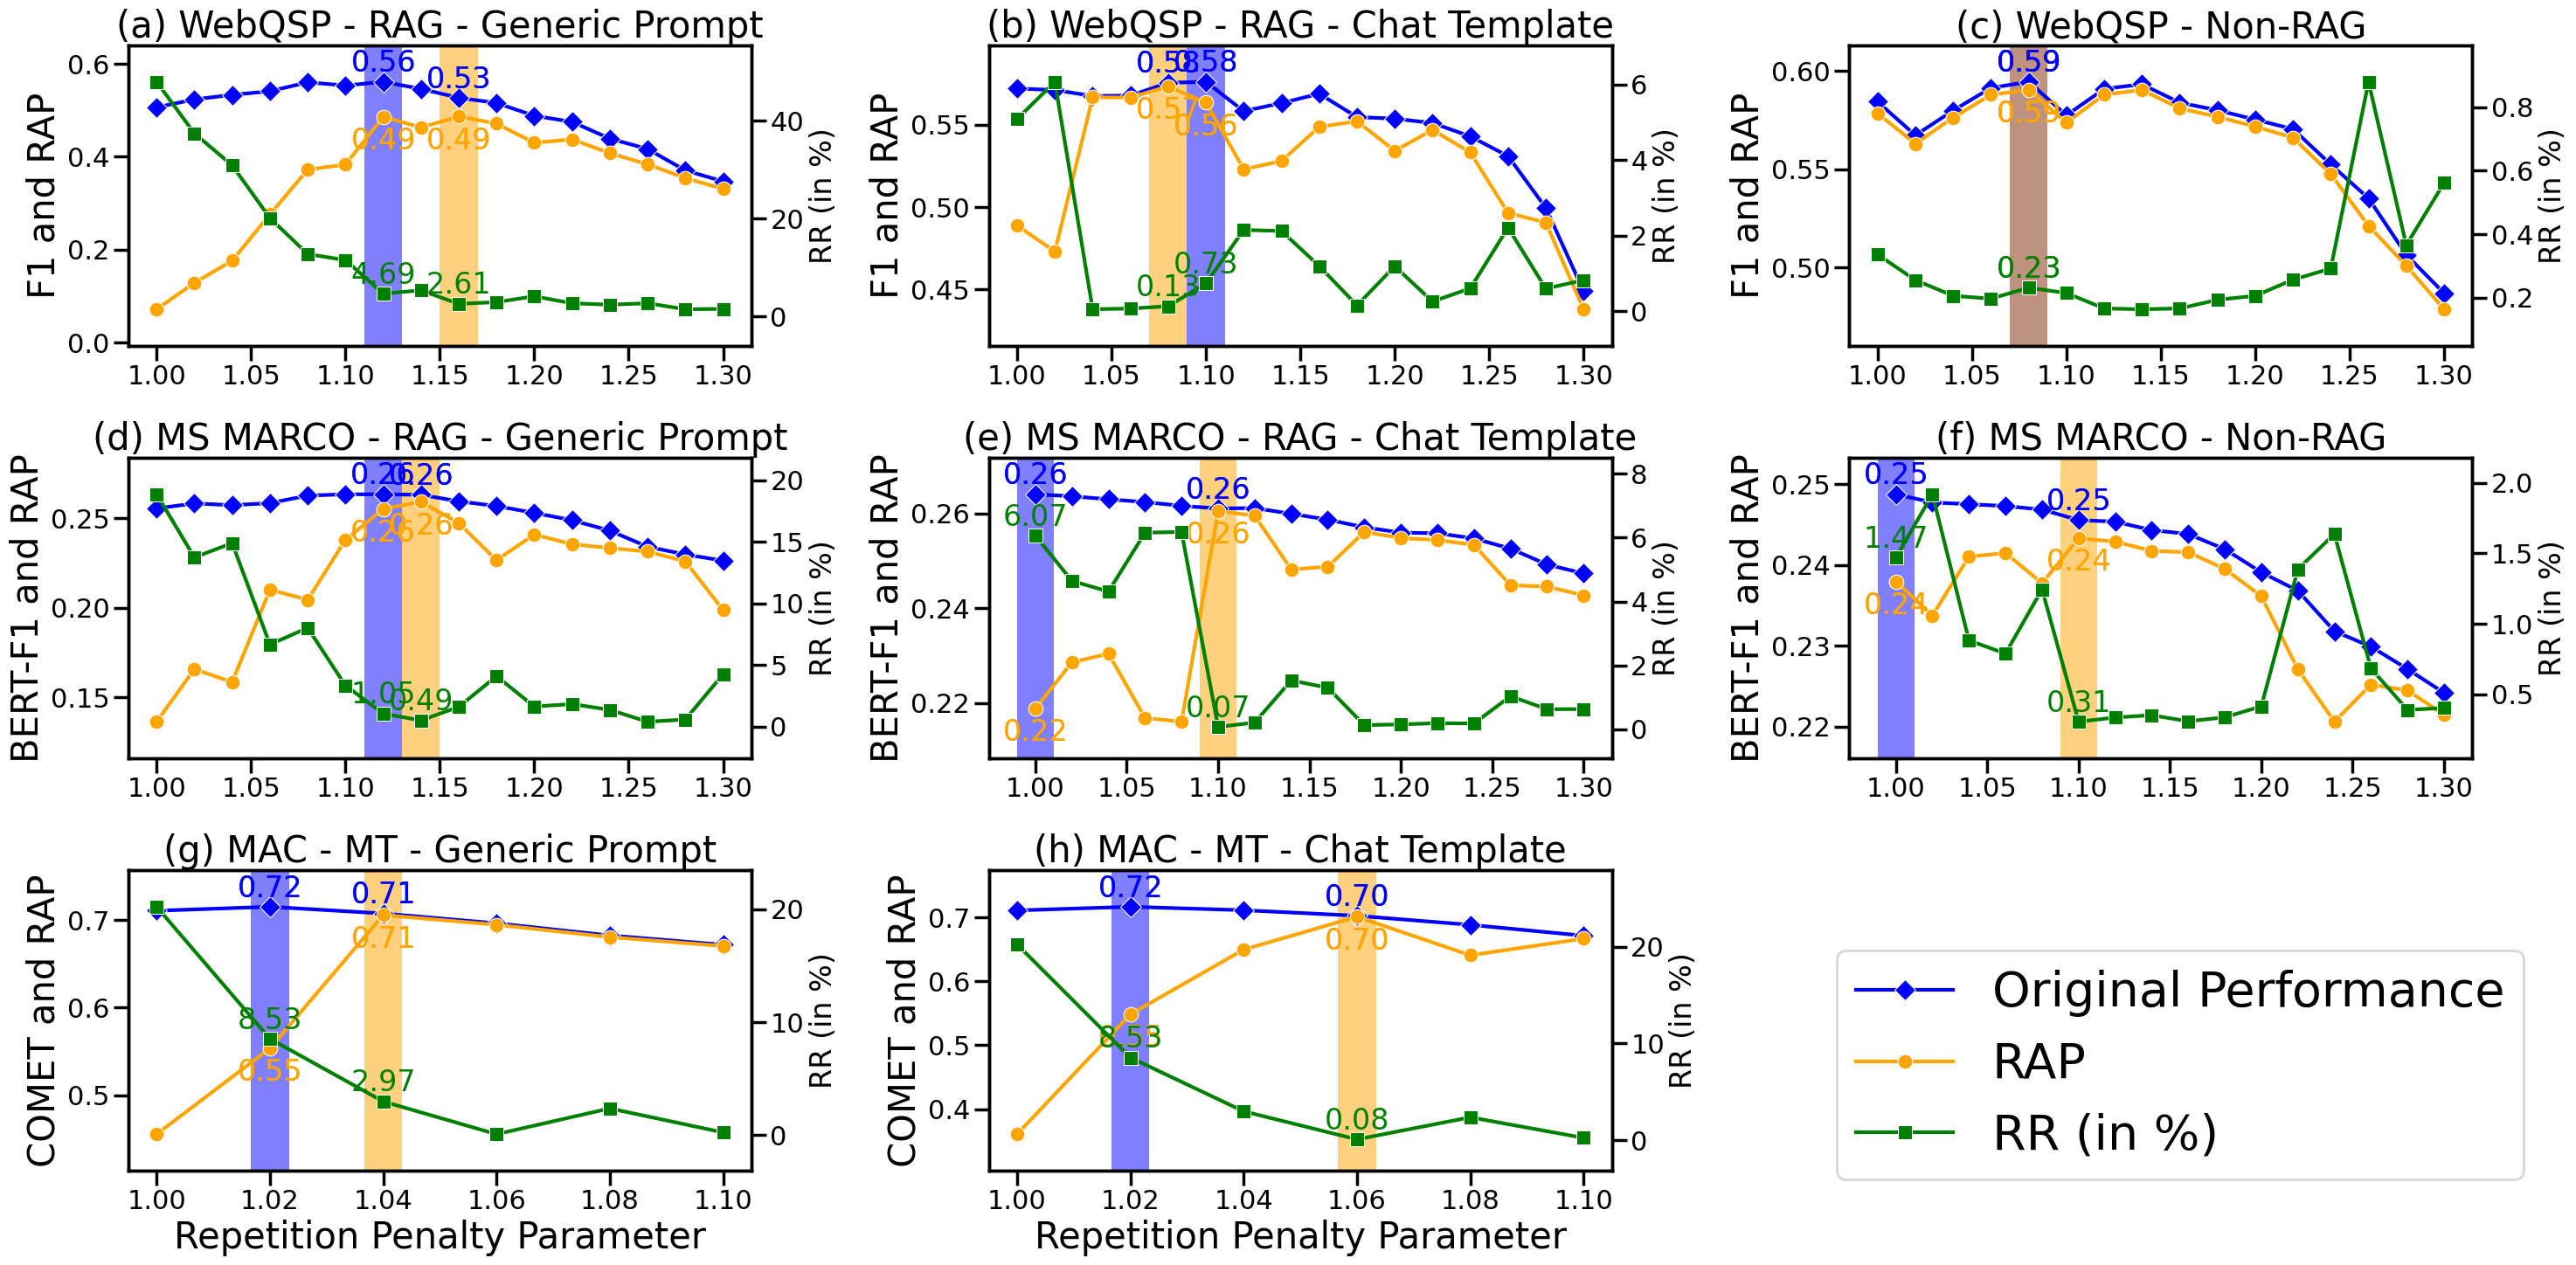
\includegraphics[width=1\textwidth]{image/performance_vs_repetition_v2.png}
    \caption[Performance vs. Repetition Trade-Off]{
    Illustrating original performance, repetition-aware performance (RAP), and repetition ratio (RR) while varying \rpp. Results are shown for Phi-3-mini in QA (Subplots (a) to (f)) and Phi-3.5-mini  in machine translation (Subplots (g) and (h)).
    % Illustrating the original performance, repetition-aware performance (RAP), and repetition ratio (RR) when varying \rpp. Results are shown for the Phi-3-mini model in QA (Subplots (a) to (f)) and the Phi-3.5-mini model in machine translation (Subplots (g) and (h)). 
    % The blue line indicates original performance (F1, BERT-F1, or COMET), the orange line represents RAP, and the green line shows RR in percentage. 
    The blue shaded region highlights the RPP for optimal original performance, while the orange region indicates the RPP for the best RAP; overlapping regions are marked in brown to show alignment.
    % Performance vs. Repetition Trade-Off. This figure shows the original performance and repetition-aware performance (RAP), and the repetition ratio (RR) when varying \rpp, across different datasets and prompt types. We showcase results from Phi-3-mini model for question answering (a-f) and Phi-3.5-mini model for machine translation (g-h) tasks. 
    % The blue line represents the original performance (F1, BERT-F1, or COMET), the orange line represents RAP, and the green line shows \rr in percentage. 
    % The blue shaded region highlights the Repetition Penalty Parameter (RPP) for the best original performance, while the orange region highlights the RPP for the best RAP. When both regions overlap, the shaded area changes to brown to indicate this alignment. 
    % Performance vs. Repetition Trade-Off. This figure shows the balance between performance and repetition reduction across different datasets and prompt types. 
    % Subplots (a-c) present results for the Phi-3-mini model on the WebQSP dataset, and subplots (d-f) show results on the MS MARCO dataset, both with different prompting strategies. Subplots (g-h) illustrate results for the Phi-3.5-mini model on the MAC machine translation task, using various prompting strategies.
    % The blue line represents the original performance (F1, BERT-F1, or COMET), the orange line represents the Repetition-Aware Performance (RAP), and the green line shows the Repetition Ratio (RR) in percentage. 
    % The blue shaded region highlights the Repetition Penalty Parameter (RPP) for the best original performance, while the orange region highlights the RPP for the best RAP. When both regions overlap, the shaded area changes to brown to indicate this alignment. 
    }
    \label{fig:performance_vs_repetition_v2}
\end{figure*}
% We conducted experiments on various datasets and models, comparing performance using both original metrics (such as F1, BLEU, and COMET) and RAP.
% }
% When tuning using conventional metrics, the objective is purely to select the value of \rpp with best performance, but that might come with serious repetition problem. Whereas, 
% Our objective is to identify the optimal \rpp that maximizes RAP by balancing model performance with the reduction of repetition in the generated content.
%
% In this section, we demonstrate the use of \rap in tuning \rpp by comparing model performance and repetition issues when tuning RPP using conventional evaluation metrics versus \rap. 
% Figure \ref{fig:performance_vs_repetition_v2} illustrates the relationship between \rpp, model performance, and repetition across different datasets and prompt strategies. We showcase results of Phi-3-mini for WebQSP and \ms, and Phi-3.5-mini for MAC. 
% The blue lines represent the original performance scores (F1 for WebQSP, BERT-F1 for MS MARCO, and COMET for MAC), the orange lines show the \rap scores, and the green lines (scaled on the right y-axis) indicate \rr in percentage. 
% The blue shaded region highlights the \rpp for the best original performance, while the orange region highlights the RPP for the best RAP. When both regions overlap, the shaded area changes to brown to indicate this alignment. 

This section demonstrates the use of RAP in tuning RPP by comparing model performance and repetition when using conventional metrics (Original Performance) versus RAP. Figure \ref{fig:performance_vs_repetition_v2} shows the relationship between RPP, performance, and repetition for Phi-3-mini on WebQSP and MS MARCO, and Phi-3.5-mini on MAC. Blue lines represent original performance (F1 for WebQSP, BERT-F1 for MS MARCO, and COMET for MAC), orange lines show RAP scores, and green lines (right y-axis) indicate RR percentages. The blue shaded area marks the RPP with the best performance based on conventional metrics, the orange marks the best RAP, and brown indicates overlap between the two.

% In most of the shown cases (except for Figure \ref{fig:performance_vs_repetition_v2}c) the best values of \rpp when tuning using original performance are different from that when tuning using \rap. For example, in Figure \ref{fig:performance_vs_repetition_v2}e, when tuning using BERT-F1, the best \rpp is 1.0 where the performance is \todo{xx}, but the repetition ratio is very high at \todo{xx\%}. Whereas, using \rap, the best \rpp is 1.1, where the performance is \todo{xx} (drop \todo{xx\%}) but the repetition ratio drop significantly to \todo{xx\%} (drop \todo{xx\%)}. This shows that tuning \rpp using \rap helps find \rpp value that minimally reduce performance while significantly lowering repetition ratio. Another example with different visualization is illustrated in Figure \ref{fig:hook}. 

In most cases (except Figure \ref{fig:performance_vs_repetition_v2}c), the optimal RPP differs when tuning for original performance versus RAP. For instance, in Figure \ref{fig:performance_vs_repetition_v2}e, tuning with BERT-F1 gives the best RPP at 1.0 with a performance of 0.264, but the repetition ratio is high at 6.07\%. With RAP, the best RPP shifts to 1.1, where performance drops by 1.1\% (drop 0.003), but the repetition ratio significantly decreases by 98.8\% (drop 6\%). This demonstrates that tuning RPP with RAP helps balance performance with reduced repetition. Another example with different visualization is illustrated in Figure \ref{fig:hook}. 
These results highlight the importance of tuning RPP to balance performance and repetition reduction, which can be achieved using RAP. The optimal RPP varies by task, dataset, and prompting strategy. 

% These results underscore the importance of carefully tuning the RPP to achieve an optimal balance between model performance and repetition reduction, that can be achieved by tuning RPP based on \rap. The optimal RPP value varies depending on the task, dataset, and prompting strategy used.

% \noindent \textbf{WebQSP}: For WebQSP with RAG-Generic Prompt (subplot a), performance remains high up to an RPP of approximately 1.12 before declining, while RR decreases significantly. In contrast, the RAG-Chat Template (subplot b) shows more stable performance across a wider range of RPP values, with lower overall repetition.

% \noindent \textbf{MS MARCO}: The results for MS MARCO (subplots d-f) follow similar trends. RAG-Generic Prompt exhibits a more pronounced trade-off between performance and repetition compared to RAG-Chat Template and Non-RAG approaches.

% \noindent \textbf{MAC}: In the MAC machine translation task (subplots g-h), increasing the RPP beyond certain thresholds (around 1.02–1.04) leads to noticeable declines in performance, while effectively reducing repetition. Both Generic Prompt and Chat Template strategies show similar trends, with higher RPP reducing repetition but negatively impacting COMET scores beyond 1.04.

% Across all datasets and strategies, there is a clear trend of decreasing RR as RPP increases. However, an excessively high RPP can lead to performance degradation. The optimal RPP, typically marked by the peak of the RAP curve (orange line) and highlighted by the orange region in the subplots, often strikes a balance between maintaining high performance and minimizing repetition.

% These results underscore the importance of carefully tuning the RPP to achieve an optimal balance between model performance and repetition reduction, which can be achieved by finding the RPP that maximizes RAP. The optimal RPP value varies depending on the task, dataset, and prompting strategy used.

% \begin{figure*}[ht]
% \centering
% 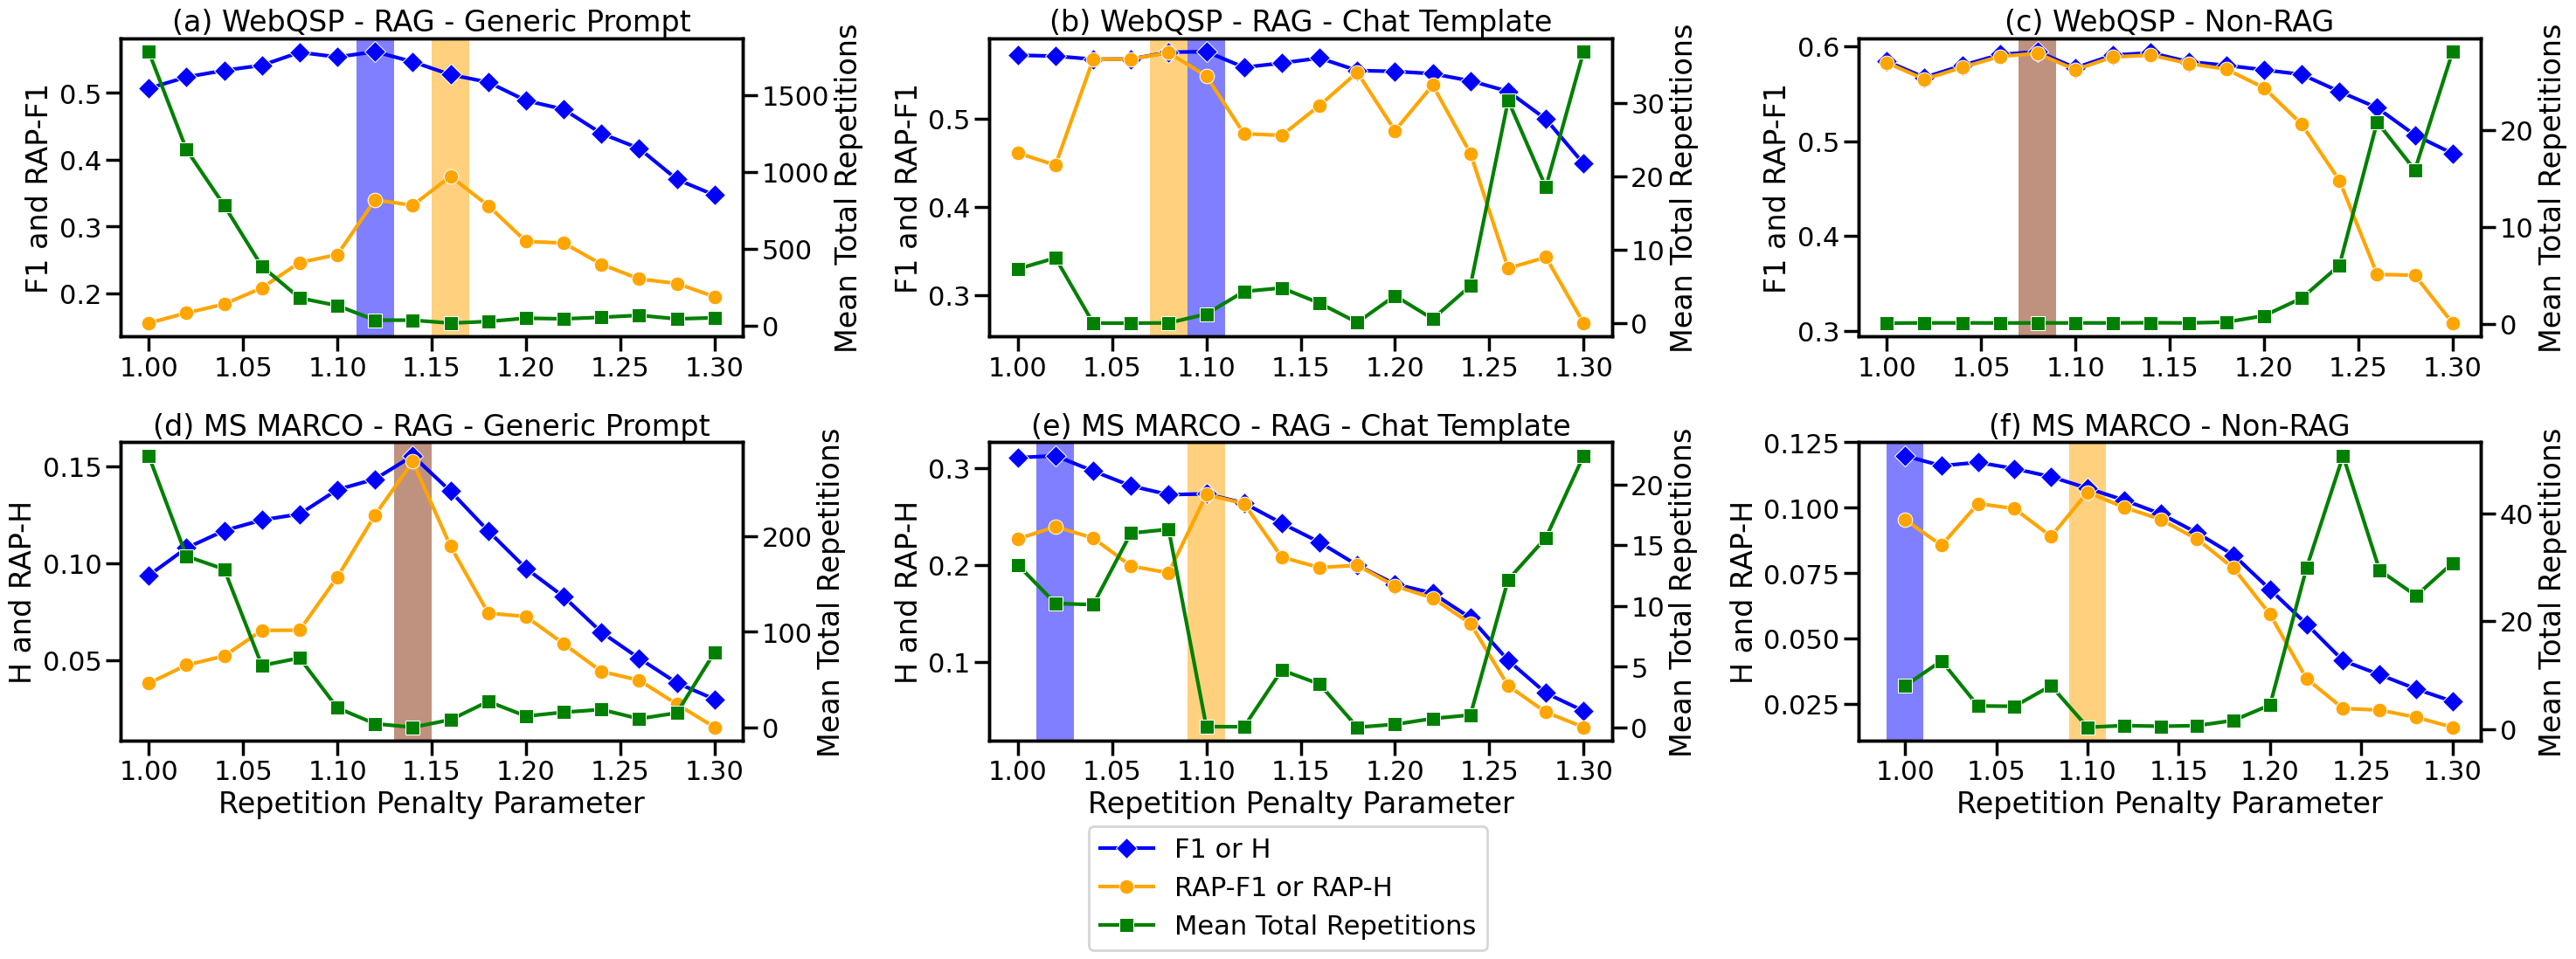
\includegraphics[width=\textwidth]{image/RPP Tuning.png}
% \caption[Performance vs. Repetition Trade-Off]{This figure illustrates the balance between performance and reducing excessive repetition for the Phi-3-mini model across various datasets and prompt types. The blue line is for F1, the orange line is for \mtr, and the green line indicates \rap. These visualizations help discern how a model’s performance and repetition behavior vary with different RPP values.}
%Performance vs. Repetition Trade-Off. This figure illustrates the balance between performance and reducing excessive repetition for the Phi-3-mini model across various datasets and prompt types. The blue lines represent the original performance (F1 or overall performance) scores, the orange lines (scaled on the right y-axis) denote the mean total repetitions (MTR) across the dataset, and the green lines indicate the repetition-aware performance (RAP), which is the original performance adjusted by $\log_{10}(10 + \alpha \times \text{MTR})$, with $\alpha$ fixed at 1 in this study. In these graphs, the blue vertical bar is centered around the RPP (Repetition Penalty Parameter) that yields the best original performance, while the orange bar is positioned at the RPP with the best RAP. In subplots (a), (b), (e), and (f), these two bars are distinctly separated, whereas in subplots (c) and (d), they overlap, resulting in a combined color (likely brown) due to the blending of blue and orange. These visualizations help discern how a model’s performance and repetition behavior vary with different RPP values, thereby aiding in determining the optimal prompts and RPP settings for any AI task.
% \label{fig:performance_vs_repetition}
% \end{figure*}



% \begin{figure*}[ht]
% \centering
% 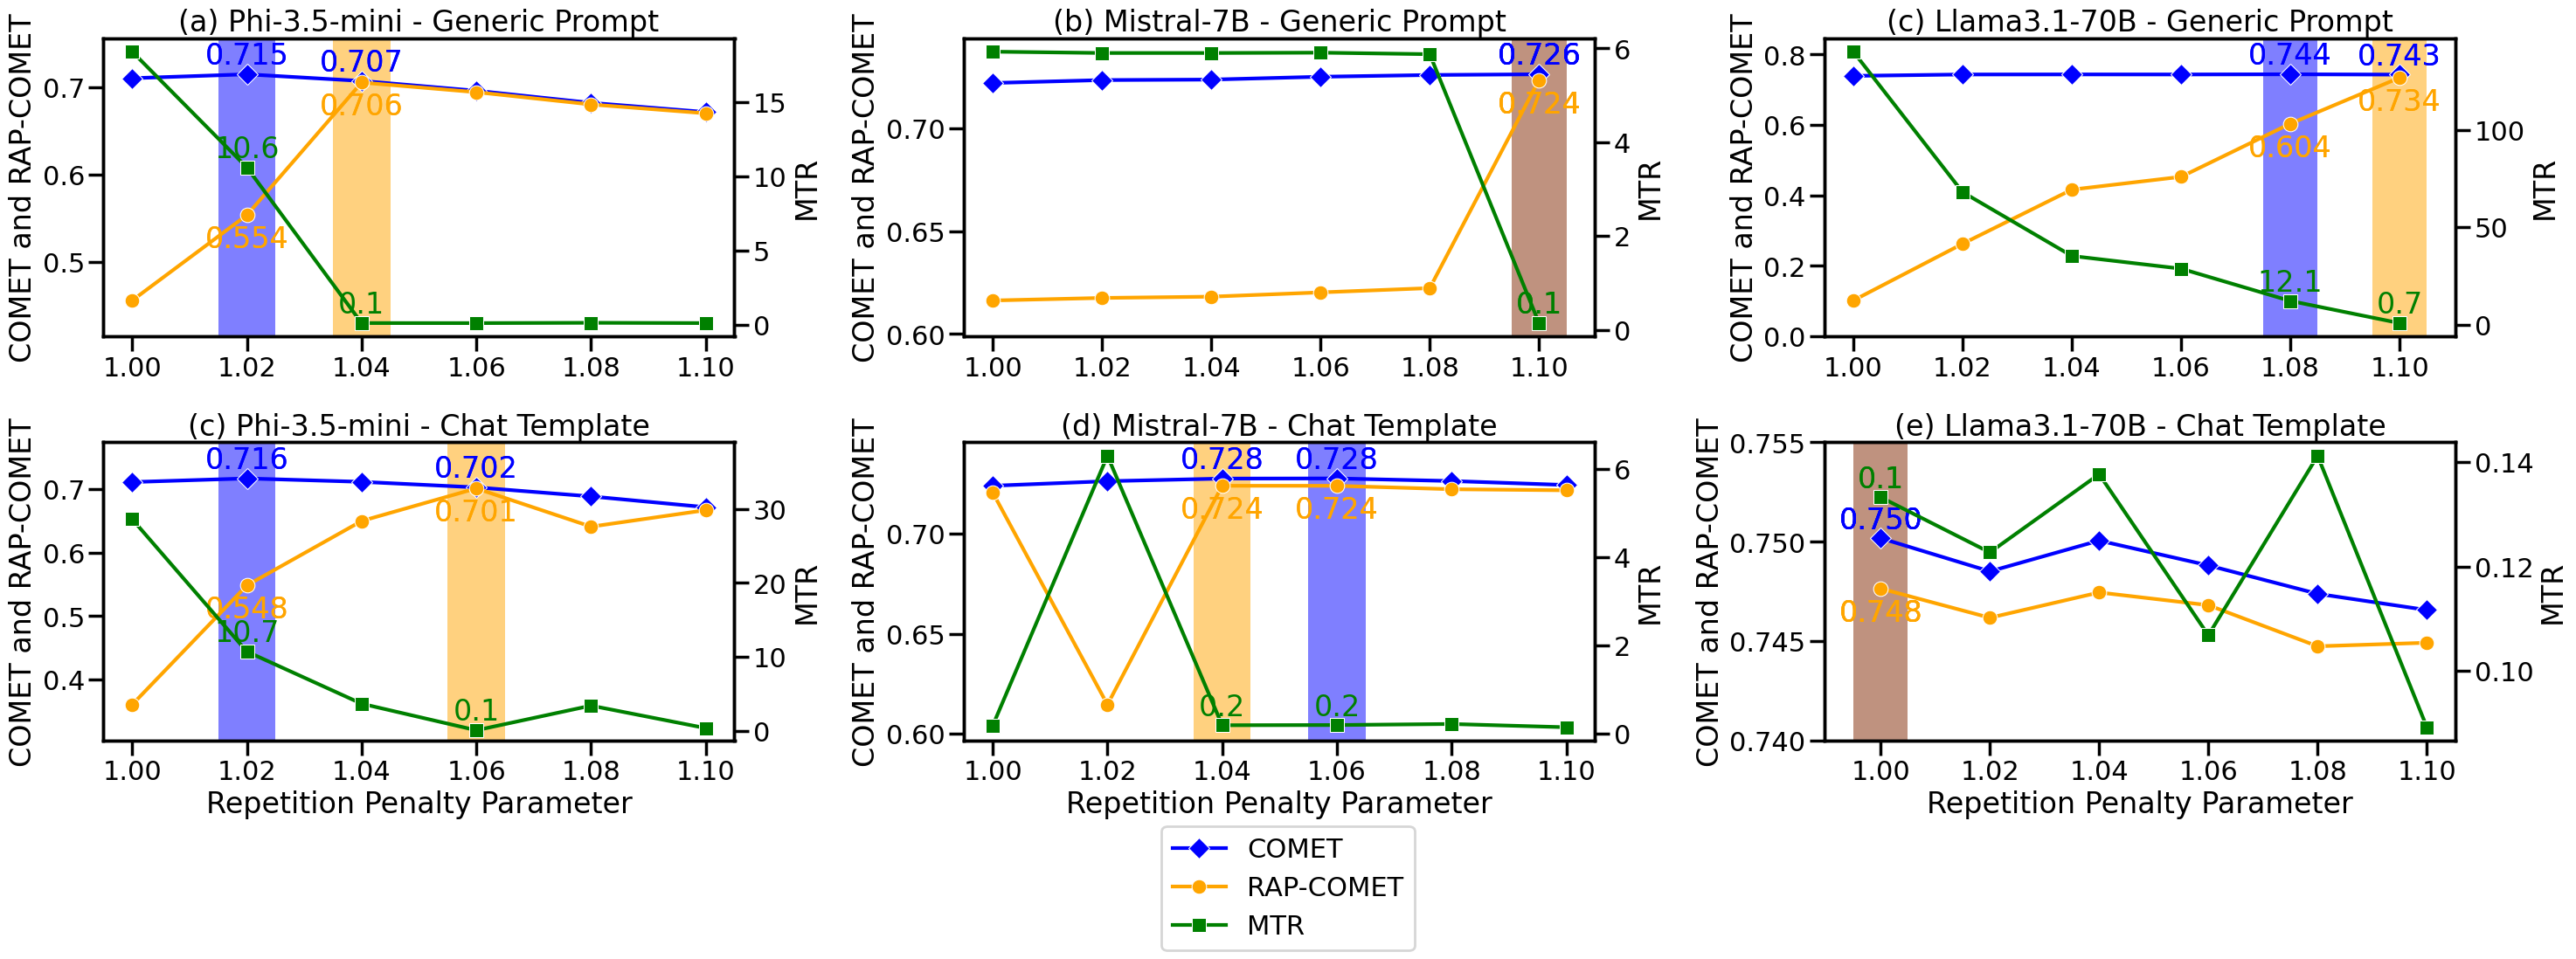
\includegraphics[width=\textwidth]{image/performance_vs_repetition_mt.png}
% \caption[Performance vs. Repetition Trade-Off for MT Tasks]{\new{Performance vs. Repetition Trade-Off for MT Tasks. This figure illustrates the trade-off between performance and the reduction of excessive repetition for the Phi-3.5-mini, Mistral-7B, and Llama3.1-70B models across both Generic Prompt and Chat Template prompt types. The blue line represents COMET, the orange line represents \mtr, and the green line represents \rap. The blue shaded region highlights the Repetition Penalty Parameter (RPP) for the best COMET performance, while the orange region highlights the RPP for the best RAP-COMET performance. When both bars overlap, the shaded region changes to brown to indicate this alignment.}}
% \label{fig:performance_vs_repetition_mt}
% \end{figure*}

% \subsection{Comparing the Best Repetition-Aware Performance of All the Models}
% \todo{@Donghao: to add table of best performance based on RAP. Maybe can use this section to compare the methods, use table. So this is to give people a sense of how the models perform, quantivatively}
% Performance Comparison based on Best \rap
% Comparing Performances of All Models selected based on best \rap. }
% Compare the Performance using tuned RPP (based on RAP)
% \input{tab_best_rpp_v2}
% \input{tab_best_rpp_v3}
% \input{tab_best_rpp_v4}

\subsection{Comparing the RAP-Tuned Performance of All Models}
Table \ref{tab:model-performance} shows the performance of the open-source LLMs after tuning \rpp using \rap. 
On \textbf{WebQSP}, Mistral-7B leads for both \raggen and \ragtem, scoring 0.609 and 0.604, respectively. However, Llama-3-70B outperforms all models in the \nonrag prompt with a high F1 score of 0.710. 
For \textbf{MS MARCO}, Gemma-1.1-2B excels in both \ragtem and \nonrag, with scores of 0.277 and 0.250, while Llama-3-70B takes the top spot in \raggen with 0.275.
In the MT task (\textbf{MAC}), Llama3.1-70B dominates both the generic prompt and chat template categories, scoring 0.743 and 0.750.
These results show that larger models like Llama-3-70B and Mistral-7B consistently achieve top performance across datasets and prompting strategies. However, mid-sized models like Gemma-1.1-2B perform competitively on specific tasks, such as MS MARCO, highlighting that model choice should be task-dependent and not solely based on model size.


% In this section, we analyze the RAP-tuned performance of various models on two different tasks: QA (Question Answering) and MT (Machine Translation). Table \ref{tab:model-performance} provides a comprehensive comparison of model performances across different datasets and prompt types. 
% For the QA task, on the \textbf{WebQSP} dataset, the \textbf{Mistral-7B} model achieves the highest performance for \raggen and \ragtem, with scores of 0.609 and 0.604, respectively. The best \nonrag performance is observed from \textbf{Llama-3-70B}, scoring an impressive 0.710.

% On the \textbf{MS MARCO} dataset, \textbf{Gemma-1.1-2B} achieves top performance for both \ragtem and \nonrag, with scores of 0.277 and 0.250, respectively. The best \raggen score for MS MARCO is achieved by \textbf{Llama-3-70B}, with a score of 0.275.

% For the MT task, \textbf{Llama3.1-70B} dominates, showing the highest performance for both \mtgen and \mttem, with scores of 0.743 and 0.750, respectively.

% These results demonstrate that larger models like \textbf{Llama-3-70B} and \textbf{Mistral-7B} consistently deliver top performance across various datasets and prompt types. However, mid-sized models such as \textbf{Gemma-1.1-2B} also perform competitively, especially on specific tasks like MS MARCO, suggesting that model selection should be guided by task-specific needs and performance trade-offs rather than size alone.




% Our proposed framework, \ours, enables tuning \rp to find the trade-off between repetition and performance, as shown in Section \ref{sec:eval_tuning}. Now, we compare the performances of all the open-source LLMs using the \rp, selected based on \rap. 
% Table \ref{tab:best_rpp} compares the performance of the open-source LLMs across two datasets, WebQSP and MS MARCO, using different prompting strategies: \raggen, \ragtem, and Non-RAG. 
% %
% For the WebQSP dataset, Mistral-7B achieves the best results with both \raggen and \ragtem strategies. In the Non-RAG category, Llama-3-70B excels. Notably, the best result for non-RAG prompting is higher than that in RAG. We argue that since we provide information retrieved from documents instead of a knowledge graph, it might not be sufficient to answer questions from KBQA task that would requires many relational information. This can be seen in the opposite observation in \ms dataset where both RAG prompting strategies obtain much higher scores than non-RAG. 
% The table also highlights the performance penalties due to repetition. For instance, Phi-3-mini using \raggen has an F1 score of 52.7, but its \rap drops to 37.5 due to repetition. A similar trend is observed with Gemma-1.1-7b under the \raggen strategy.
% We also present the best results tuned based on the original F1 scores for \webqsp (denoted as [MODEL-NAME]-F1). This is to demonstrate the potential impact of not considering repetition when tuning \rp. We observed that using our framework, \ours, significantly reduces the repetition issue, with minimal changes in overall performance. For instance, with Llama-2-7B \raggen, an \rp of 1.0 yields the best F1 score of 60.1 but has a high repetition rate of 78.48 on average. However, using \ours, we can select the \rp of 1.06 which drastically reduces the mean total repetition to 0.01, while still achieving a comparable F1 score of 58.9. Several other similar cases are highlighted in blue text, illustrating the effectiveness and benefits of our framework in balancing repetition and performance.
% \todo{to revise, remove framework, to use metric}
% Our proposed framework, \rap, allows tuning \rp to balance repetition and performance, as shown in Section \ref{sec:eval_tuning}. We compare the performances of all open-source LLMs using the selected \rp based on \rap.
% Table \ref{tab:best_rpp} shows the performance of these LLMs across WebQSP and MS MARCO datasets with different prompting strategies: \raggen, \ragtem, and Non-RAG. For WebQSP, Mistral-7B performs best with \raggen and \ragtem, while Llama-3-70B excels in Non-RAG. Interestingly, the best Non-RAG result is higher than RAG, likely because document retrieval may not provide sufficient relational information needed for KBQA tasks. This contrasts with the MS MARCO dataset, where both RAG strategies outperform Non-RAG.
% The table also shows the performance penalties due to repetition. For example, Phi-3-mini using \raggen has an F1 score of 52.7, but its \rap drops to 37.5 due to repetition, a trend also seen with Gemma-1.1-7b under \raggen.
% We also present the best results tuned based on original F1 scores for \webqsp, denoted as [MODEL-NAME]-F1, to show the impact of not considering repetition when tuning \rp. Using our metric, \rap, significantly reduces repetition with minimal performance changes. For instance, with Llama-2-7B \raggen, an \rp of 1.0 yields an F1 score of 60.1 but has a high repetition rate of 78.48. However, with \ours, an \rp of 1.06 reduces repetition to 0.01, still achieving an F1 score of 58.9. Other similar cases are highlighted in blue, demonstrating our framework’s effectiveness in balancing repetition and performance.

% For the MS MARCO dataset, the performance trends shift. The Llama-3-70B model stands out under the \raggen strategy, achieving the highest F1 (33.7) and RAP (33.7) scores. Gemma-2B and Mistral-7B perform best for the RAG-Chat Template and Non-RAG strategies, respectively. There are significant drops from RAG to non-RAG performances. This is due to the difficulty of \ms questions and the high quality of relevant data provided in RAG prompts for \ms. 
% Overall, for both WebQSP and MS MARCO, most models exhibit zero or very low repetition (MTR), demonstrating the effectiveness of \ours in choosing \rp for balancing repetition and performance.



% \subsection{RAG with Chat Template vs Generic Template}
% \subsection{RAG (template or generic, depending on if we can have more results for template WebQSP) with non-RAG}
% \subsection{Repetitions of different settings}
% Can show the differences between different repetition detection methods (method 1 vs method 3 vs method 3.2)
% \subsection{Adjusted results vs original}

% \subsection{Ablation study of what Penalty function should be used?}
% \todo{@Donghao: to add figure + discussion of penalty functions}

% \todo{move to appendix}
% In this section, we qualitatively evaluate the quality of KBQA evaluation generated by Gemini (Section \ref{sec:gemini}). Table \ref{tab:gemini_eval} show examples of output from Llama 3-70B for five \webqsp questions and the corresponding evaluation from Gemini. In the first example, Gemini is able to extract answer-item is ``Lawrence E. Roberts'', and generate the correct mapping between predicted answer and ground-truth answer, this leads to a correct evaluation. Another correct evaluation is obtained in the second example. However, sometimes Gemini fails to extract correct information from generated text. For example, in the third question, Gemini extracted ``Elizabeth Bowes-Lyon'' is also a predicted answer-item, although from the LLM response, we can see that this is not. This leads to giving this answer with 0.5 precision only, hurting the overall performance of the LLM. Another such cases can be seen in the fifth question where Gemini extracted many keywords from the LLM response, this makes the final score is very low, even though by reading the response, we see that the predicted answer was correct. 
% To better understand the quality of our LLM-based KBQA evaluation method, we randomly select 100 samples from the experiment results of Llama-3-70B Non-RAG as this setting obtains the best performance on \webqsp. Then, we ask a human user if the user agree with Gemini's evaluation (similar to the analysis we have done above). The agreement is \textbf{89.0\%}. This shows that although not perfect, our LLM-based KBQA evaluation method has some level of reliability which can be used for KBQA evaluation task.  
% \subsection{Evaluate the Quality of Gemini's Evaluation} 
% \label{sec:eval_gemini}
% To evaluate the quality of our LLM-based KBQA evaluation method, we randomly selected 100 samples from the experiment results of Llama-3-70B Non-RAG, as this setting achieved the best performance on WebQSP. We then asked a human user to review and agree with Gemini’s evaluation (similar to the analysis described above). The agreement rate was 89.0\%, indicating that while not perfect, our LLM-based KBQA evaluation method demonstrates a level of reliability that can be utilized for automatically evaluating LLM responses in the KBQA task. For more details of the actual output from Gemini, please see Section \ref{sec:a_gem} in Appendix. 



% E.g., manually check X samples. Or how? Can mention some question are returned NONE for evaluation. Pick 50 questions, ask human (3 of us?, 3 * 50 or 3*20) to do the same task as Gemini, then we measure precision, recall of Gemini. \todo{to select 150 questions from Llama 3 70B Non RAG, assign 50 to each of us}

% \subsection{Further Discussions}

\subsection{How Severe can Repetition be?}
\begin{figure}[ht]
    \centering
    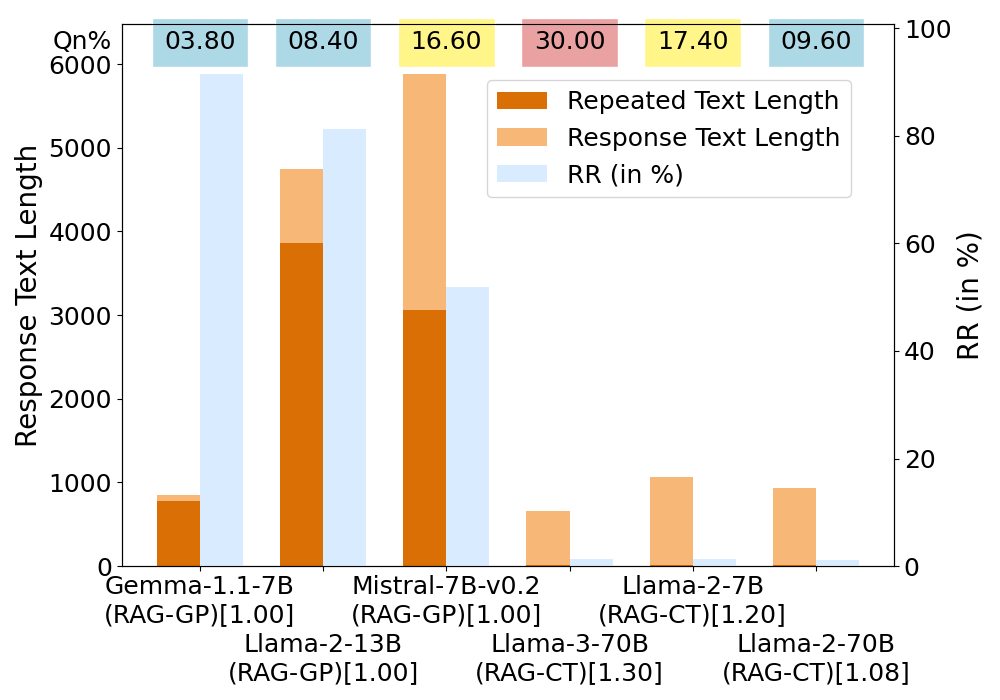
\includegraphics[width=1\linewidth]{image/chart_02_mm.png}
    \caption{
    Severity of repetition. Colored squares above indicate the percentage of repetitive responses. X-label contains model, prompting method, and tuned \rpp.
    % , and the x-label includes the model, prompting method, and tuned value for \rpp. 
    % The severity of repetition. The leftmost three models have the highest RR for \ms, while the rightmost three have the lowest, along with the repetition ratio (y-axis-right) and text length (y-axis-left). Colored squares above each point indicate the percentage of repeated responses, and the x-label includes the model, prompting method, and tuned value for \rpp. 
    % 
    % The severity of repetition. The leftmost three models show the Top-3 highest RR for MS MARCO, while the rightmost three display the lowest. The ratio of repeated text length to text length is also visualized. Colored squares above each point indicate the percentage of repeated questions, with blue, yellow, and red squares marking values below 10\%, between 10-20\%, and above 20\% respectively. The x-label indicates the model, the prompting method, and the RP of the RR. The chart for other models and dataset can be viewed in the appendix.
    }
    \vspace{-1em}
    \label{fig:msmarco_top3}
\end{figure}
In our experiments, the length of text repeated can account for up to 97.85\% of the overall text output, while the proportion of responses with repetition across the entire dataset can reach 41.27\%. Figure \ref{fig:msmarco_top3} shows the top-3 highest and lowest RR for \ms. Colored squares above each point indicate the percentage of repeated responses, with blue, yellow, and red squares marking values below 10\%, between 10-20\%, and above 20\%, respectively. Notably, while Gemma-1-1.7B (RAG-GP) has only 3.8\% of responses with repetition, the repeated text case is very severe as it makes up 91.53\% of the overall answer length. In contrast, 30\% of Llama-3-70B (RAG-CT)'s responses contains repetition, but the repeated text only constitutes 1.29\% of the overall length. The length of repeated content can also be substantial. For instance, Llama-2-13B generated repeated content that averaged around 4,000 characters. 

\subsection{Ablation Study: the Effects of Different Penalty Functions}
\begin{figure}[ht!]
    \centering
    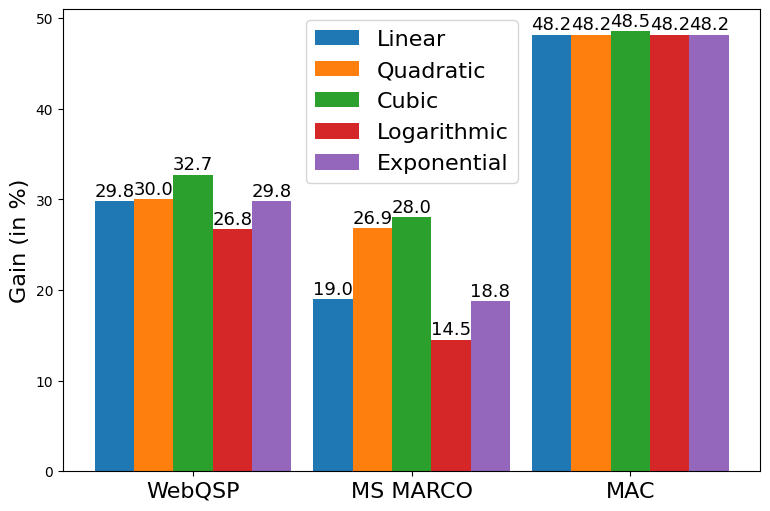
\includegraphics[width=\linewidth]{image/ablation_study.png}
    \caption{Gains across different penalty functions. \textit{Cubic} penalty obtains the best gains across three datasets.}
    \label{fig:ablation_study}
    % \vspace{-1em}
\end{figure}

We now present an ablation study to evaluate the impact of different formulas for the penalty function $F(\rr)$ on \rap (Equation \ref{eq:rap}). We consider five options including \textit{Linear}, \textit{Quadratic}, \textit{Cubic}, \textit{Logarithmic}, and \textit{Exponential} where the penalty are $1-\rr$, $(1-\rr)^2$, $(1-\rr)^3$, $\text{log}_{2}(2-\rr)$, and $e^{-\rr}$, respectively. 
%
We compare the \textit{Gain} achieved with each repetition penalty formula. For a model, \textit{Gain} is defined as the difference between the reduction in repetition and the performance drop when tuning RPP using original performance versus RAP. It reflects how much repetition decreases (i.e., gain) relative to the performance loss when tuning RPP with RAP. The higher \textit{Gain}, the better. 
%
Figure~\ref{fig:ablation_study} shows the \textit{Gain} scores for each formula across the three datasets. The \textit{Gain} for a dataset is calculated by averaging the \textit{Gain} values from all models and prompting strategies. 
% The results show that the \textit{Cubic} penalty consistently achieves the highest gain across all datasets (32.7\% for WebQSP, 28.0\% for MS MARCO, and 48.5\% for MAC), indicating it offers the best balance between reducing repetition and maintaining performance. Notably, all penalty formulas perform similarly well on MAC, with gains around 48\%, suggesting the choice of penalty is less critical for tasks where performance is less sensitive to repetition reduction like MAC. These findings support using the \textit{Cubic} penalty for the RAP metric as it provides a strong balance across varied datasets and tasks.
The results show that the \textit{Cubic} penalty consistently achieves the highest gains across all datasets (32.7\% for WebQSP, 28.0\% for MS MARCO, and 48.5\% for MAC), offering the best balance between reducing repetition and maintaining performance. These findings recommend the \textit{Cubic} penalty for the RAP metric, as it performs well across diverse datasets and tasks.

% The results show that \textit{Cubic} penalty consistently achieves the highest gain across all three datasets (32.7\% for WebQSP, 28.0\% for MS MARCO, and 48.5\% for MAC). This indicates that the cubic function provides the most optimal balance between reducing repetition and preserving model performance.
% Interestingly, all penalty functions perform similarly well on MAC, with gains hovering around 48\%. This suggests that the choice of penalty function may be less critical for tasks or datasets where performance is less sensitive to repetition such as MAC. 
% These findings support our choice of the \textit{cubic} penalty function for the RAP metric, as it provides a robust balance between repetition reduction and performance preservation across diverse datasets and tasks.




% The results highlight several key findings:

% \noindent \textbf{Superiority of Cubic Penalty:} The \textit{cubic} penalty function consistently achieves the highest gain across all three datasets (32.74\% for WebQSP, 28.03\% for MS MARCO, and 48.54\% for MAC). This indicates that the cubic function provides the most optimal balance between reducing repetition and preserving model performance.

% \noindent \textbf{Consistency Across MAC Dataset:} Interestingly, all penalty functions perform similarly well on the MAC dataset, with gains hovering around 48\%. This suggests that the choice of penalty function may be less critical for tasks or datasets where performance is less sensitive to repetition, such as in the MAC dataset.

% \noindent \textbf{Variation Across Datasets:} The \textit{logarithmic} and \textit{exponential} penalty functions exhibit varied performance across datasets. While they perform relatively well on the MAC dataset, they lag behind the polynomial functions (linear, quadratic, and cubic) on both WebQSP and MS MARCO, indicating that the effectiveness of these functions may be task- or dataset-dependent.

% These findings support our choice of the \textit{cubic} penalty function for the RAP metric, as it provides a robust balance between repetition reduction and performance preservation across diverse datasets and tasks.




% The \textit{Gain} is defined as the difference of repetition ratio deduction and performance deduction, i.e., how much repetition drop versus how much performance drops, the large \textit{Gain}, the better. 



% \rap integrates \rr into the overall model performance by applying a penalty function to repetition in the generated content, as defined in Equation~\ref{eq:rap_generic}.

% \begin{equation}
%     \text{RAP} = P \times f(x)
%     \label{eq:rap_generic}
% \end{equation}

% Where $P$ is the performance metric (e.g., F1 score), $f(x)$ is a penalty function, and $x = 1 - \text{RR}$.

% We evaluated the following penalty functions:

% \begin{align}
%     f_{\text{linear, quadratic, cubic}}(x) &= x^n \quad \text{where} \, n \in \{1, 2, 3\} \\
%     f_{\text{logarithmic}}(x) &= \log_2(1 + x) \\
%     f_{\text{exponential}}(x) &= e^{x - 1}
% \end{align}

% We define the \textit{gain} as:

% \begin{equation}
%     \text{Gain} = \frac{\text{RR}_{\text{original}} - \text{RR}_{\text{RAP}}}{\text{RR}_{\text{original}}} - \frac{P_{\text{original}} - P_{\text{RAP}}}{P_{\text{original}}}
% \end{equation}

% Where $\text{RR}_{\text{original}}$ and $P_{\text{original}}$ are the repetition ratio and performance at the best performance-tuned RPP, while $\text{RR}_{\text{RAP}}$ and $P_{\text{RAP}}$ are the corresponding values at the best RAP-tuned RPP.

% Figure~\ref{fig:ablation_study} presents the results of this ablation study, showing the gains achieved across three datasets—WebQSP, MS MARCO, and MAC—for each penalty function. The goal was to maximize the gain, i.e., to achieve the highest reduction in repetition with minimal performance degradation.

% \begin{figure}[ht]
%     \centering
%     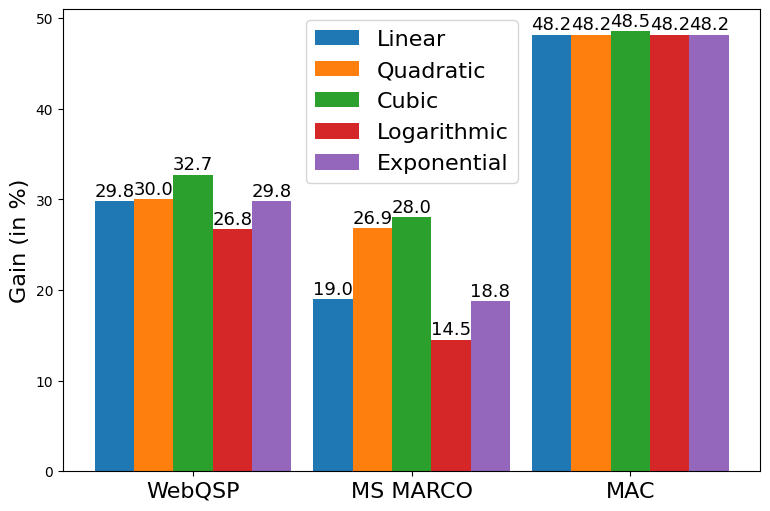
\includegraphics[width=\linewidth]{image/ablation_study.png}
%     \caption{Gains across different penalty functions on three datasets (WebQSP, MS MARCO, and MAC). The evaluated penalty functions include \textit{linear}, \textit{quadratic}, \textit{cubic}, \textit{logarithmic}, and \textit{exponential}.}
%     \label{fig:ablation_study}
% \end{figure}

% The results highlight several key findings:

% \noindent \textbf{Superiority of Cubic Penalty:} The \textit{cubic} penalty function consistently achieves the highest gain across all three datasets (32.74\% for WebQSP, 28.03\% for MS MARCO, and 48.54\% for MAC). This indicates that the cubic function provides the most optimal balance between reducing repetition and preserving model performance.

% \noindent \textbf{Consistency Across MAC Dataset:} Interestingly, all penalty functions perform similarly well on the MAC dataset, with gains hovering around 48\%. This suggests that the choice of penalty function may be less critical for tasks or datasets where performance is less sensitive to repetition, such as in the MAC dataset.

% \noindent \textbf{Variation Across Datasets:} The \textit{logarithmic} and \textit{exponential} penalty functions exhibit varied performance across datasets. While they perform relatively well on the MAC dataset, they lag behind the polynomial functions (linear, quadratic, and cubic) on both WebQSP and MS MARCO, indicating that the effectiveness of these functions may be task- or dataset-dependent.

% These findings support our choice of the \textit{cubic} penalty function for the RAP metric, as it provides a robust balance between repetition reduction and performance preservation across diverse datasets and tasks.